\documentclass[12pt]{book}
\usepackage[T1]{fontenc}
\usepackage[utf8]{inputenc}
\usepackage[spanish]{babel}
\usepackage{amsmath}
\usepackage{MnSymbol}
\usepackage{wasysym}
\usepackage{multicol}
\setlength{\columnsep}{1cm}
\usepackage[margin=2.5cm,left=3cm, includehead]{geometry}
\usepackage{graphicx}
\usepackage{float}
\usepackage{fancyhdr}
\usepackage{cancel}
\usepackage{pgf,tikz}
\usepackage{mathrsfs}
\usetikzlibrary{arrows}
\usepackage{amsthm}
\usepackage{amsfonts}
\renewcommand{\baselinestretch}{1.5}
\usepackage{cite}

% Theorems and definitions
\theoremstyle{plain}
\newtheorem{theorem}{Teorema}[chapter]
\newtheorem{exercise}[theorem]{Ejercicio}
\newtheorem{proposition}[theorem]{Proposición}
\newtheorem{definition}[theorem]{Definición}
\newtheorem{corollary}[theorem]{Corolario}
\newtheorem{obsservation}[theorem]{Observación}
\newtheorem{example}[theorem]{Ejemplo}
\newtheorem{notation}[theorem]{Notación}
\newtheorem{lemma}[theorem]{Lema}

%% NEW Comands
\newcommand{\R}{\mathbb R}  
\newcommand{\N}{\mathbb N}  
\newcommand{\Z}{\mathbb Z}  
\newcommand{\mf}[1]{\mathbf{#1}}

\begin{document}
\title{Tesis primera parte.}
\author{Jorge Ballote}
\thispagestyle{plain}
\pagenumbering{Roman}
% \input{agradecimientos.tex}
\tableofcontents
% \input{resumen.tex}
\newpage
\pagenumbering{arabic}

    %%%%%%%%%%%%%%%%%%%% CHAPTER  %%%%%%%%%%%%%%%%%%%%%%%
    %------------------------------------- Preeliminares-------
    \chapter{Preliminares}
    Antes de poder hablar del Aprendizaje profundo, o de Redes Neuronales Convolucionales, es importante sentar las bases matemáticas y computacionales requeridas para su estudio. A continuación, se presentan algunas definiciones y resultados conocidos de temas tales como cálculo, álgebra y ciencias de la computación.
    \section{Resultados de Cálculo y Álgebra lineal}
    \begin{definition}[Polinomio de Taylor]
        Sea $f$ una función $n$ veces diferenciable, y sean $$a_k = \frac{f^{(k)}(a)}{k!}.$$
        Definimos el Polinomio de Taylor de grado $n$ para $f$ en $a$ como
        $$P_{n,a}(x) = a_0 + a_1(x-a) + \cdots + a_n(x-a)^n.$$
    \end{definition}
    El polinomio $P_{n,a}(x)$ ha sido definido de manera que $P_{n,a}(a) = f^{(k)}(a)$ para $0\leq k \leq n$.
    \begin{definition}
        Sea $f$ una función tal que $P_{n,a}(x)$ existe, definimos el término  residual $R_{n,a}(x)$ como 
        \begin{equation}
            R_{n,a}(x) = f(x) - P_{n,a}(x).
        \end{equation} 
    \end{definition}
    \begin{theorem}[Teorema de Taylor]
        Supóngase que $f^{(1)}$, $f^{(2)}$, ..., $f^{(n+1)}$ están definidos en $[a,x]$. Entonces 
        \begin{equation}
            R_{n,a}(x) = \frac{f^{n+1}(t)}{(n+1)!}(x-a)^{n+1}
        \end{equation}
        para algún $t\in (a,x)$.
    \end{theorem}

    \begin{definition}
        Sea $x$ una característica en $\mathbb R^{h\times w\times d}$. La vectorización de $x$, denotada $X = \text{vec}(x)$ es un vector en $\mathbb R^{hwd}$ tal que 
        \begin{equation}
            X_{(k-1)hw + (i-1)w + j} = x_{i,j,k},
        \end{equation}
        para todos $i=1,2, ..., h$, $j = 1, 2, ..., w$, $k= 1,2,..., d$.
    \end{definition}
    \textcolor{red}{explicar que es una característica (feature). Además, en la definición de convolución uso una imagen $I$, tal vez sea más consistente escribir una característica $x$.}
    \begin{definition}
        Una matriz $H$ es llamada \textsl{Circulante} si es de la forma
        \begin{equation}
            H = \begin{bmatrix}
                h_0 & h_1 & \cdots & h_{N-1} \\
                h_{N-1} & h_0 & \cdots & h_{N-2} \\
                \vdots & \vdots &  & \vdots \\
                h_1 & h_2 & \cdots & h_{0} \\
            \end{bmatrix}
        \end{equation}
        ya que $H$ queda completamente determinada con la primera fila, es posible escribir $H = \text{circ}(h_0, ..., h_{N-1})$.
    \end{definition} 
    \begin{definition}
        \label{doubly_circulant_matrix}
        Una matriz $H$ es llamada \textsl{Doblemente Circulante por Bloques} si es de la forma
        \begin{equation}
            H = \begin{bmatrix}
                H_0 & H_1 & \cdots & H_{N-1} \\
                H_{N-1} & H_0 & \cdots & H_{N-2} \\
                \vdots & \vdots &  & \vdots \\
                H_1 & H_2 & \cdots & H_{0} \\
            \end{bmatrix} = \text{circ}(H_0, ..., H_{N-1})
        \end{equation}
        dónde $H_i = \text{circ}(h_{i,0}, ..., h_{i, N-1})$.
    \end{definition}
    \begin{definition}
        Sean $A$ y $B$ dos conjunto. El producto cartesiano $A \times B$ se define como
        \begin{eqnarray}
            A \times B &= \{(a,b) : a\in A \text{ y } b\in B\}.
        \end{eqnarray}
        De igual manera sean $A_1, ..., A_s$ son conjuntos, el producto cartesiano se define como
        \begin{equation}
            A_1\times A_2 \times ... \times A_s = \{(a_1,..., a_s): a_i\in A_i, \quad i= 1,...,s\}.
        \end{equation}
        De modo natural, se define $A^n :=  A \times A \times ... \times A$ donde $A$ se repite $n$ veces.
    \end{definition}
    A su vez, nos es conveniente destacar otra notación
    
    \begin{notation}
        Sean $a_1, ..., a_n\in \mathbb N$. Definimos $\mathbb R^{a_1 \times a_2 \times ... \times a_s} := \mathbb R^{a_1} \times ... \times \mathbb R^{a_s}$
    \end{notation}

    \begin{definition}
        Sean $u,v\in \mathbb R^n$, el producto punto de $u$ con $v$ denotado como $u\cdot v$ es
        \begin{equation}
            u_1v_1 + u_2+v_2 + ... + u_nv_n
        \end{equation}
        donde $u_i$ y $v_i$ representan la $i$-ésima entrada de los vectores $u$ y $v$ respectivamente.
    \end{definition}

    \begin{definition}
        Una función vectorial es una función de la forma $f:\mathbb R \to \mathbb R^n$.
    \end{definition}

    \begin{definition}
        La derivada $f'$ de una función vectorial $f: \mathbb R \to \mathbb R^n$ se define como
        \begin{equation}
            f'(t) = \lim_{h\to 0} \frac{f(t+h)- f(t)}{h\to 0}.
        \end{equation}
    \end{definition}
    Sin embargo, en la práctica, no es necesario utilizar la definición, pues 
    \begin{theorem}
        La derivada $f'$ de una función vectorial $f = (f_1, f_2, ..., f_n)$, con $f_i: \mathbb R \to \mathbb R$ es
        \begin{equation}
            f'(t) = (f_1'(t), f_2'(t), ..., f_n'(t)).
        \end{equation}
    \end{theorem}
    \begin{definition}[Gradiente]
        Sea $f: \mathbb R^n \to \mathbb R$. El gradiente de $f$ es el vector conformado por las derivadas parciales en cada una de las $n$ variables:
        \begin{equation}
            \nabla f = \left(\frac{\partial f}{\partial x_1}, ..., \frac{\partial f}{\partial x_n}\right).
        \end{equation}
    \end{definition}
    \begin{proposition}[Regla de la cadena]
        Sea $f: \mathbb R^n \to \mathbb R$ y $v: \mathbb R \to R^n$. Es posible hallar la derivada de la composición.
        \begin{equation}
            \frac{d}{dt}(f\circ g) = \nabla f \cdot  v'(t)
        \end{equation}
    \end{proposition}

    \begin{definition}[Notación O-grande (Big O)]
        Sean $f$ y $g$ funciones $f,g:\mathbb N \to \mathbb R^+$. Decimos que $f(n) = \mathcal O(g(n))$ si existen enteros positivos $c$ y $n_0$ tales que para cualquier entero $n\geq n_0$,
        \begin{equation}
            f(n) \leq cg(n).
        \end{equation}
        Cuando $f(n) = \mathcal O(n)$, decimos que $g(n)$ es una cota asintótica superior de $f(n)$,
    \end{definition}

    %------------------------------------- Vision computacional -------
    \section{Visión Computacional}
    El problema de clasificación de imágenes, pertenece a la rama de la visión computacional. La siguiente definición de imagen fue extraída del libro \cite{computer_vision}.
    \begin{definition}
        Una \textsl{imagen digital} es una función $I:  D \subset \mathbb Z^2 \to U$. Dónde el domino es un rectángulo con coordenadas enteras $D = [1,M]\cap \mathbb Z \times [1,N] \cap \mathbb Z$. La terna $(x,y,u)$ se conoce como pixel.
        \begin{itemize}
            \item Cuando las imágenes son a escala de grises se tiene que $U=[0,255]\cap \mathbb Z$. Es decir que $u\in U$ es un valor de 0 a 255.
            \item Si las imágenes son a color, consideramos $U=([0,255]\cap \mathbb Z)^3$. Es decir que $u\in U$ es una terna de valores de 0 a 255. A cada entrada de la terna se conoce como un canal de color.
        \end{itemize}
    \end{definition}
    Es posible representar una \textsl{imagen digital} $I$ como un \textsl{Tensor}, de la siguiente manera.
    \begin{equation}
        T_{i,j,k} = u_k, \quad u = I(i,j)
    \end{equation}

    \textcolor{red}{Definir en algún punto lo que es un tensor}
    %------------------------------------- Inteligencia artificial y aprendizaje profundo -------    
    \section{Inteligencia artificial y Aprendizaje profundo}
    El \textsl{Aprendizaje de Máquina} es un caso particular de la inteligencia artificial, en donde la máquina aprende de los datos proporcionados. Para entender este concepto es importante definir qué significa aprender \cite{Mitchell}.
    \begin{definition}
        Se dice que un programa de computadora aprende de la experiencia $E$ respecto a un conjunto de tareas $T$ y medida de rendiminto $P$ si el rendimiento en las tareas en $T$, medido con $P$ mejora gracias a la experiencia $E$.
    \end{definition}
    Ya que aprender, implica mejorar el rendimiento en una tarea específica, sería bueno remarcar algunas de las tareas más comunes en el campo del aprendizaje automático.
    \begin{enumerate}
        \item \textbf{Clasificación.} Consiste en que el modelo reconozca que elementos pertenecen a ciertas clases, teniendo en cuenta sus características. Por ejemplo, distinguir perros de gatos, o en el caso de este proyecto podría ser diferenciar entre polen y polvo
        \item \textbf{Regresión.} Aquí lo que se busca es usar la información existente para tener una predicción aproximada de algún escalar. Por ejemplo, predecir el precio de una casa, dadas sus características (ubicación, número de cuartos, antiguedad, etc).
        \item \textbf{Agrupamiento (Clustering).} Este es un méto de aprendizaje no supervisado, que tiene como objetivo detectar similitudes entre las instancias, y separarlas en grupos de elementos similares entre sí.
    \end{enumerate}
    
     %------------------------------------- Overfitting y Underfitting -------    
    \subsection{Sobreajusto y Desajuste}
    En el aprendizaje automático, nuestro modelo aprende de un conjunto de entrenamiento $\mathcal X$. Sin embargo, una vez que nuestro modelo ha aprendido ¿Cómo podemos determinar que aprendió correctamente o que desempeñó de manera satisfactoria su tarea? La manera de determinar que nuestro modelo es bueno, es probando su capacidad de hacer predicciones con datos que no haya utilizado durante el entrenamiento. Para ello, es necesario un conjunto de imágenes nuevas $\mathcal X'$ al cual llamaremos conjunto de prueba. 

    El proceso de entrenamiento consiste en optimizar una función en nuestro conjunto $\mathcal X$, donde es posible encontrar una medida de error, la cual se conoce como \textsl{error de entrenamiento}. Sin embargo, nuestro objetivo es reducir el error en nunestro conjunto de prueba, el cuál se denomina \textsl{error de prueba}. El desempeño correcto de un modelo en el conjunto de prueba se conoce como \textsl{generalización} y por ello el error de entrenamiento también es conocido como \textsl{error de generalización}

    Asumimos que los elementos en nuestros conjuntos de datos son \textsl{independientes} y además que el conjunto de entrenamiento y el de prueba están \textsl{identicamente distribuidos}, lo cual se conoce como las suposiciones IID. Con estas suposiciones y debido a la naturaleza del entrenamiento, se espera que el error de prueba se reduzca a la par que el error de entrenamiento, y lo más normal es que el error de prueba sea mayor que el de entrenamiento.

    Sin embargo, el conjunto de funciones que puede adoptar un modelo, depende de la cantidad de parámetros que este tenga, lo cual se conoce como \textsl{capacidad}. Con una capacidad suficiente, siempre es posible hacer un mapeo perfecto entre entradas y etiquetas. Sin embargo, no es la función que se adapte mejor a los datos de entrenamiento la que es más conveniente, sino la que generalice mejor. Cuando la diferencia entre el error de entrenamiento y el error de generalización se acrescenta se dice que el modelo sufre de un \textsl{sobreajuste}. Cuando la capacidad de un modelo es muy reducida, puede ocurrir que no sea posible reducir el error de entrenamiento con lo que el modelo sufre de un \textsl{desajuste}.
    % imagen de sobreajuste y desajuste. 

    \subsection{Regularización}
    Cuando se entrena un modelo, son necesarias dos partes: 
    \begin{enumerate}
        \item Optimización: En donde, se busca minimizar la función de costo.
        \item Generalización: Es importante que las predicciones de nuestro modelo sean aplicables con datos que no hayan sido vistos en el entrenamiento.
    \end{enumerate}
    Sin embargo, no es fácil conseguir ambos objetivos simultáneamente. En vez de priorizar alguno de los dos, la \textsl{regularización} pretende lograr que se satisfagan ambos de la mejor manera. Es decir, \textsl{la regularización es cualquier modificación en el algoritmo de entrenamiento, cuyo objetivo sea reducir el error de generalización, pero no el error de entrenamiento}.
    % \begin{example}(Weight Decay)
        
    % \end{example}
    % \begin{figure}[H]
    %     \includegraphics{regularization.png}
    % \end{figure}
    \textcolor{red}{Insertar imágenes con ejemplos}
    Una de las formas más comunes de regularizar un modelo que aprende la función $f(x, \theta)$, es agregando una penalización $R(\theta)$ a la función de costo, considerando $\theta$ como los parámetros.
    \subsection{Función de activación.
    }
    Con la intención de ampliar el conjunto de funciones que un modelo puede predecir, en cada capa de nuestras redes neuronales, se compone una función no lineal denominada \textsl{función de activación}. En caso de no incluirla, el conjunto de funciones disponibles para nuestro modelo serían sólo funciones lineales, debido a que la composición de dos funciones lineales $L_1$ y $L_2$ da lugar a otra función lineal $L_1 \circ L_2$.

    Existen muchos ejemplos de funciones no lineales. En un principio se usaban funciones suaves como la función \textsl{sigmoidal} $(1+\exp(x))^{-1}$, la tangente hiperbólica $\tanh(x)$, o la función \textsl{Softplus} $\dfrac{1}{\beta} \log(1+ \exp(\beta x))$. Sin embargo, las tendencias modernas prefieren las funciones no suaves como es el caso de la más popular \textsl{ReLU} $\max(x,0)$.

    \begin{figure}[H]
        \centering
        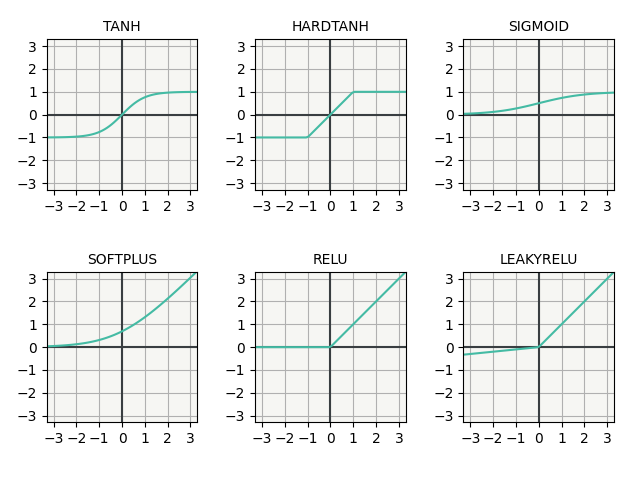
\includegraphics[width=6in]{../cap1_preliminares/src/activations.png}
        \caption{\textcolor{red}{Usar una imagen propia}}
    \end{figure}
    
    % Transferemcia de aprendizaje
    \subsection{Transferencia de aprendizaje}
    La transferencia de aprendizaje en el campo del aprendizaje profundo, es un concepto motivado por la psicología, que se basa en usar conocimientos adquiridos para cierta tarea $A$, con el objetivo de aprender alguna tarea $B$. Por ejemplo, si una persona sabe bailar salsa, posiblemente pueda usar esos conocimientos para aprender a bailar bachata. 

    En la mayoría de los casos, los conjuntos de datos tienen una cantidad limitada de imágenes etiquetadas. Una posible solución a este problema, es usar \textsl{aprendizaje semisupervisado}, el cuál requiere algunas imágenes etiquetadas, pero también se pueden usar varias imágenes no etiquetadas. Sin embargo, incluso los conjuntos de datos no etiquetados, pueden ser insuficientes. Cuando se tienen conjuntos de datos muy pequeños, es posible apoyarse de modelos pre-entrenados con millones de imágenes, con la esperanza de que las características aprendidas anteriormente, sean de utilidad en el nuevo conjunto de datos.
    % Conjuntos desbalanceados
    \subsection{Conjuntos desbalanceados}
    Cuando se enfrenta el problema de clasificación, digamos con $m$ clases, uno esperaría que tengamos suficientes ejemplos de cada clase. Más aún, para que nuestro modelo no tenga ningún sesgo por ninguna clase, es preferible que en nuestro conjunto de entrenamiento, todas las clases tengan una cantidad similar de ejemplos. De lo contrario, nuestro modelo podría ser entrenado con demasiados elementos de una clase particular $mathcal C$, y tendería a clasificar muchos elementos en la clase $\mathcal C$. Además de esto, si nuestro conjunto de prueba también está desbalanceado, no se vería reflejado el sesgo en métricas comunes como la exactitud y la precisión.

    \begin{definition}
    \label{balanced}
        Sea $\mathcal C$ un conjunto de datos, cuyas clases son $\mathcal C_1, ..., \mathcal C_m$. Un conjunto de datos se dice balanceado con tolerancia de $\epsilon$ si 
        \begin{equation}
            1-\epsilon \leq \frac{|C_i|}{|C_j|} \leq 1 + \epsilon, \quad i,j = 1,2, ..., m.
        \end{equation}
        Un conjunto es desbalanceado bajo la tolerancia $\epsilon$ si no es balanceado.
    \end{definition}
    Para efectos prácticos, diremos que un conjunto balanceado con tolerancia $\epsilon = 0.1$
    \begin{example}
        Supóngase ahora que dada una lista de características, se quisiese clasificar a las personas infectadas de COVID-19. En México el índice de positividad es del $17\%$ \cite{}. Por lo que si se toman todas las pruebas realizadas tendríamos la siguiente razón:
        \begin{equation}
            \frac{|C_{Neg}|}{|C_{Pos}|} = 4.8823 > 1.1.
        \end{equation}
        El tamaño de la clase de pruebas negativas es casi 5 veces mayor al tamaño de la clase de pruebas positivas. Por consiguiente, estaríamos en presencia de un conjunto de datos desbalanceado.
    \end{example}
    \begin{figure}[H]
        \centering
        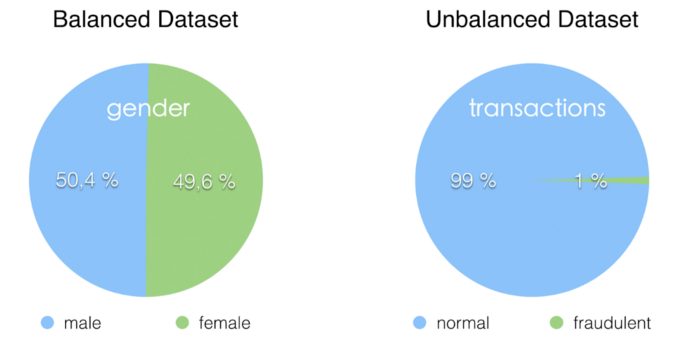
\includegraphics[width=6in]{../cap1_preliminares/src/unbalanced.png}
        \caption{\textcolor{red}{Usar una imagen propia}}
    \end{figure}
    \subsubsection{Afrontar un problema con un conjunto desbalanceado}
    La forma principal de lidiar con un conjunto desbalanceado es, valga la redundancia \textsl{balancear el conjunto}. Es decir, forzar al datset a tener clases cuyos tamaños coincidan. Para conseguir esto, es posible seguir distintas estrategias.
    \begin{itemize}
        \item \textbf{Submuestreo.} Consiste en tomar la classe \textcolor{red}{mayoritaria} (La clase con menor número de elementos) y eliminar algunas instancias, de modo que el conjunto quede balanceado. La manera más sencilla, es tomando elementos aleatorios del conjunto. Sin embargo, esto puede retirar instancias que contengan información esencial, por lo que sólo es recomendable en caso de tener un conjunto de datos muy grande.

        Otros algoritmos, heurísticos se basan en dos diferentes modelos de teoría de ruido. Algunos investigadores consideran que las instancias cercanas a los márgenes de clasificación de dos clases, son consideradas ruido. Por otro lado, algunos investigadores consideran que las instancias presentes en vecindades de varias etiquetas distintas, se pueden considerar como ruido. De modo que en lugar de remover elementos aleatorios, estas estrategias implican hacer el submuestreo tomando en cuenta únicamente las instancias que no sean ruido.

        \item \textbf{Sobremuestreo.} Al igual que en el submuestreo, existe el sobremuestreo aleatorio, el cual se basa en crear copias idénticas de las instancias de la clase minoritaria, de modo que la nuestra clase minoritaria alcance la magnitud del resto de clases. Al aplicar este método, se incrementa el riesgo de sobreajustar el modelo. 

        Otras algoritmos de sobremuestreo, generan instancias sintéticas para incremantar la cantidad de datos en una clase. Existen diversas formas de conseguir esto. Una posibilidad, es usando el aumento de datos únicamente en la clase minoritaria, permitiendo rotaciones, traslaciones y otras transformaciones. Existe también algoritmos como el VAE, SMOTE, MSMOTE. 

    \end{itemize}

    \begin{figure}[H]
        \centering
        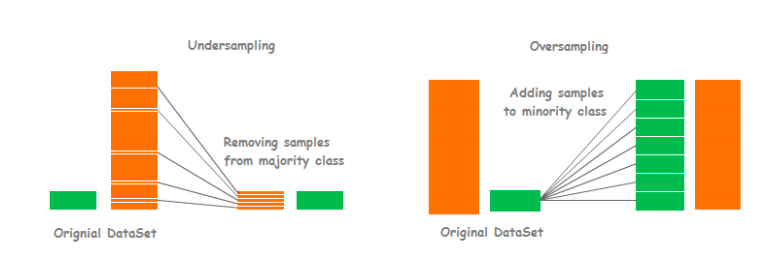
\includegraphics[width=6in]{../cap1_preliminares/src/undersampling_oversampling.png}
        \caption{\textcolor{red}{Usar una imagen propia}}
    \end{figure}

    \subsubsection{Métricas distintas a la exactitud}
    Como hemos mencionado antes, la exactitud no debe ser la única métrica a considerar en un problema con conjunto de datos desbalanceado. La razón es simple: es posible obtener una muy buena exactitud sin realmente hacer predicciones de nuestra clase minoritaria.
    \begin{example}
        \label{diff_metrics}
        Si tenemos un conjunto de datos con dos clases, tal que una clase $C_1$ representa el $99\%$ de las instancias, y la clase $C_2$ el $1\%$ restante. Si tomamos el clasificador $f: \mathcal C \to \{1,2\}$, $f(x) = 1$. Claramente nuestra exactitud sería del $99\%$, pero las predicciones de nuestra clase minoritaria aciertan un $0\%$ de las veces.
    \end{example}{}
    Una forma de sobrellevar el efecto visto en el ejemplo \ref{diff_metrics} es analizando el desempeño del clasificador para cada clase por separado y luego hacer un promedio. En el caso de nuestro ejemplo todas las instancias que en verdad pertenecen a la clase 1, fueron clasificadas correctamente (1.0), y las instancias que pertenecen a la clase 2, fueron clasificadas todas incorrectamente (0.0). Con lo con esta nueva métrica tendríamos una puntuación de $\frac{1.0 + 0.0}{2} = 0.5$. En el capítulo \ref{experimentos} se definen formalmente las métricas relevantes para este trabajo. Sin embargo, las métricas más utilizadas para este tipo de problemas son las siguientes:
    \begin{itemize}
        \item Confussion matrix: De ésta matriz, se pueden obtener métricas útiles tales como Specificity, Sensitivity, Precision, Recall
        \item F1-score: La media armónica de precision y recall
        \item ROC curves
        \item Logloss
        \item Kappa: Exactitud de la clasificación, normalizada por el desbalance de clases en nuestros datos.
    \end{itemize}

    % Perceptrón {}{}
    \subsection{Redes completamente conectadas}

    \subsection{Clasificación de imágenes}
    Para poder clasificar las imágenes, los algoritmos de inteligencia artificial extraen características importantes de una imagen. ¿Qué puede ser tomado en cuenta como importante? Podría pensarse que las esquinas, los bordes u otros detalles. Sin embargo, los algoritmos de aprenizaje automático suelen ser cajas negras, dónde las caraceterísticas relevantes de una imagen, a simple vista no parezcanr
    \begin{definition}[Característica]
        Una característica $x$ es un elemento de $\mathbb R^{w\times h\times d}$, dónde $w,h\in \mathbb N$ representan las dimensiones espaciales y $d$ la cantidad de canales.
    \end{definition}

    \section{Notas del capítulo}
    \begin{enumerate}
        \item  Añadir la referencia: A Comprehensive Survey on Transfer Learning
        \item Falta terminar la sección de transferencia de aprendizaje
        \item Uso términos como exactitud y precisión, cuándo estos se definen en la última sección.
        \item Añadir la referencia de la población de Hombres y Mujeres en el ejemplo 1 de conjuntos desbalanceados
        \item Añadir referencia de positividad de Covid en México en el ejepmlo 2 de conjuntos desbalanceados.
    \end{enumerate}
 %%%%%%%%%%%%%%%%%%%%%%%%% CHAPTER %%%%%%%%%%%%%%%%%%%%%%%%%%%%%%%%
\chapter{Redes Neuronales Convolucionales}


Las primeras Redes Neuronales Convolucionales (CNN por sus siglas en inglés) datan de 1980  por Fuksihima \cite{firstCnn} y 1998 desarrollada por Yann Lecun \cite{lecunCnn}. Sin embargo, no fue hasta el 2012 con la introducción de la AlexNet \cite{alexnet} que la comunidad científica empezó a destinar recursos considerables a su estudio. Con el propósito de entender a profundidad a las CNNs, definiremos lo que es una convolución. Para un estudio más detallado es posible consultar \cite{CNNdefinition,deeplearningbook}. 

%------------------------------ 1.Convoluciones -----------------------
\section{Convoluciones}
La convolución es una operación binaria que tiene muchas aplicaciones en los campos de matemáticas y física \cite{convolution_for_quaternion}, tales como álgebra lineal y procesamiento de señales. En cuánto a Inteligencia Artificial se refiere, las convoluciones son utilizadas para construir arquitecturas invariantes ante las traslaciones \cite{convolution_invariance}. A continuación se definen matemáticamente las convoluciones y en la Sección \ref{section_cnn} se definen las CNNs.
 \begin{definition}[Convolución]
    \label{convolution_definition}
     Sean $f,g : \R \to \R$. La convolución de $f$ con $g$, denotada como $f * g$ se define como:
     $$(f*g)(t) = \int_{0}^t f(\tau)g(t-\tau)d\tau$$
 \end{definition}

 Uno de las propiedades de las convoluciones es que son invariantes ante las traslaciones \cite{convolution_invariance}.
\begin{proposition}
    Sea $T_af$ el operador de traslación definido por $T_af(t) = f(t+a)$. Se tiene que 
    \begin{equation}
        T_a(I*K) = (T_af)*K.
    \end{equation}
\end{proposition}

 Sin embargo la Definición \ref{convolution_definition} no es muy práctica para los paradigmas computacionales, pues  las limitaciones físicas nos obligan discretizar la integral a modo de suma. Además, las imágenes son funciones cuyo dominio es subconjunto de $\mathbb R^2$. Por lo que es necesario extender la definición \ref{convolution_definition} a más de una dimensión.
 \begin{definition}[Convolución de una imagen con un kernel]
     Sea $I$ una imagen y $K$ un kernel bidimensional. La convolución de $I$ con $K$ es la imagen $(I*K)$ definida como:
     $$(I*K)(i,j) = \sum_m\sum_n I(m,n)K(i-m,j-n).$$ 
 \end{definition}
 En varias bibliotecas de aprendizaje automático se implementa una correlación cruzada en lugar de una convolución. La única diferencia entre una correlación cruzada y una convolución es la orientación del Kernel. En este trabajo, adoptaremos la convención usual de referirnos a las correlaciones como convoluciones. 
 \begin{definition}
     Sea $I$ una imagen y $K$ un kernel bidimensional. La correlación cruzada de $I$ con $K$ es la imagen definida por 
     $$(I*K)(i,j) = \sum_m\sum_n I(i+m,j+n)K(m,n).$$ 
 \end{definition} 

 \begin{figure}[H]
     \centering
     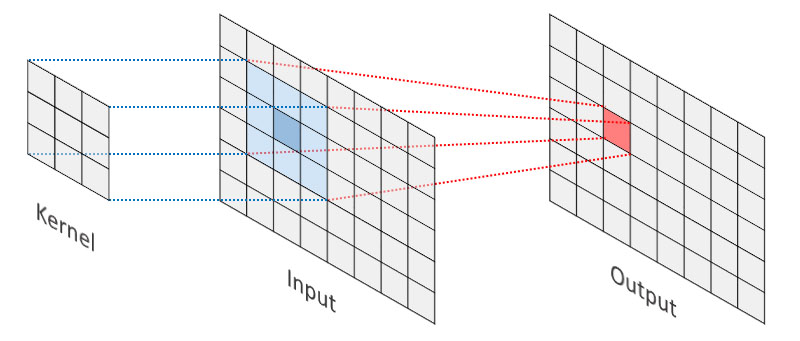
\includegraphics[width=4in]{../src/ch1convolution.png}
     \caption{Representación gráfica de una convolución. Para cada posición del Kernel sobre la imagen, se realiza una multiplicación \textsl{entrada por entrada} del Kernel y la un conjunto de pixeles de la imagen, del mismo tamaño que el Kernel.} 
 \end{figure}
 Cuando calculamos la correlación cruzada, desplazamos el kernel 1 pixel a la vez. Sin embargo, es posible aumentar la cantidad de pixeles que avanza el kernel en cada iteración. A esto se le conoce como tamaño de paso 

 
 %------------------------------ Stride -----------------------
 \subsection{Stride}
 \begin{definition}
    Sea $x$ una característica, y $K$ un kernel. Denotamos la correlación cruzada con tamaño de paso $a$, de la siguiente manera 
    \begin{equation}
        (I*K)|_a = (I*K)(i,j) = \sum_m\sum_n I(i+m+a \cdot i,j+n+a \cdot j)K(m,n)
    \end{equation}
 \end{definition}
 Debido a lass convenciones en la notación, a la correlación cruzada con tamaño de paso $a$, también se le llamará \textsl{convolución con tamaño de paso $a$}.

 \begin{figure}[H]
    \centering
    \includegraphics[width=4in]{../cap2_CNNs/src/stride_convolution.png}
    \caption{Convolución con tamaño de paso 2} 
\end{figure}
 %------------------------------ Convoluciones con múltiples canales -----------------------
 \subsection{Convoluciones con múltiples canales}
 Las imágenes RGB suelen tener 3 canales, cada uno representa la intensidad de cada color: rojo, verde y azul respectivamente. Más aún, en las redes modernas, se suelen hallar características con múltiples canales, en cada capa. Es por esto, que es imperativo definir convoluciones para características con más de un canal.
 Antes de definir lo que es una convolución para múltiples canales, definiremos un concepto más general de \textsl{kernel}.
 \begin{definition}
    Decimos que un kernel $K$ multicanal tiene $d_1$ canales de entrada y $d_2$ canales de salida cuando $K\in \mathbb R^{k\times k\times d_1 \times d_2}$.
    $$K = \left(
        \begin{matrix}
            K_{1,1} & K_{1,2} & \cdots & K_{1,d_2} \\
            K_{2,1} & K_{2,2} & \cdots & K_{2,d_2} \\
            \vdots & \vdots & \ddots & \vdots \\
            K_{d_1,1} & K_{d_1,2} & \cdots & K_{d_1,d_2} \\
        \end{matrix}
    \right)$$  
    Cada $K_{i,j}\in \mathbb R^{k\times k}$ representa un subfiltro de $K$.
 \end{definition}
 Cuando no exista ambiguedad, los kernel multicanal también pueden ser denotados como kernel.
 \begin{definition}
    Sean $x\in \mathbb R^{h \times w \times d_2}$ una característica y $K\in \mathbb R^{k\times k \times d_1\times d_2}$ un kernel con $d_1$ canales de entrada y $d_2$ canales de salida. Denotamos la convolución 2D de $x$ y $K$ como:
    \begin{equation}
        y_j := \sum_{i=1}^{d_1} K_{i,j} \otimes x_i, \quad j = 1, ..., d_2.
    \end{equation}

 \end{definition}
 \begin{figure}[H]
    \centering
    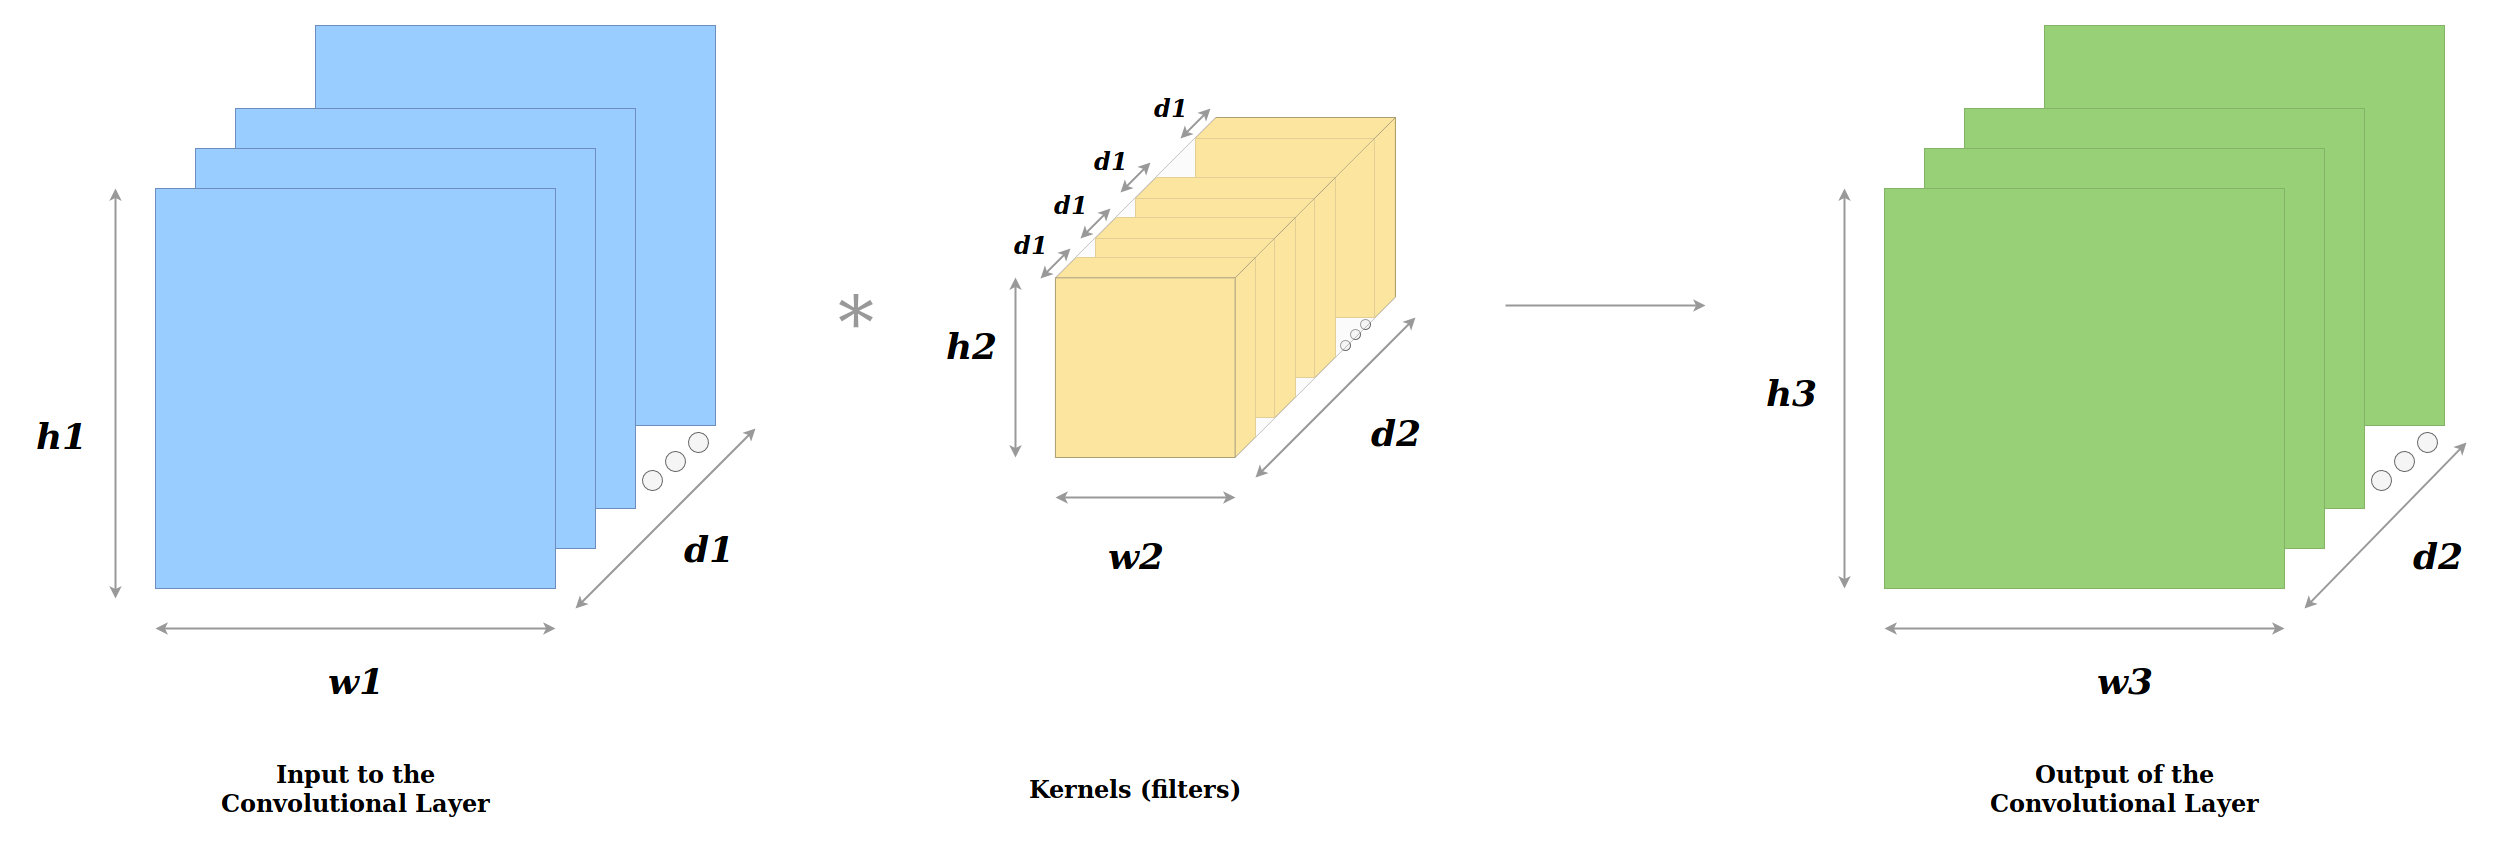
\includegraphics[width=4in]{../cap2_CNNs/src/conv2d.png}
    \caption{La convolución 2D puede ser usada con características de $d_1$ canales y devolver una característica de $d_2$ canales.} 
\end{figure}
 %------------------------------ Padding -----------------------
 \subsection{Padding}
 Debido a que la operación de convolución utiliza  pixeles adyacentes, no es posible calcular los bordes de la imagen resultante. Suponiendo que se tiene una imagen de $n\times n$ y un kernel de $k\times k$ con $k$ impar. Sólo es posible calcular la parte interior de la imagen resultante de tamaño $n-k+1$.
 \begin{figure}[H]
    \centering
     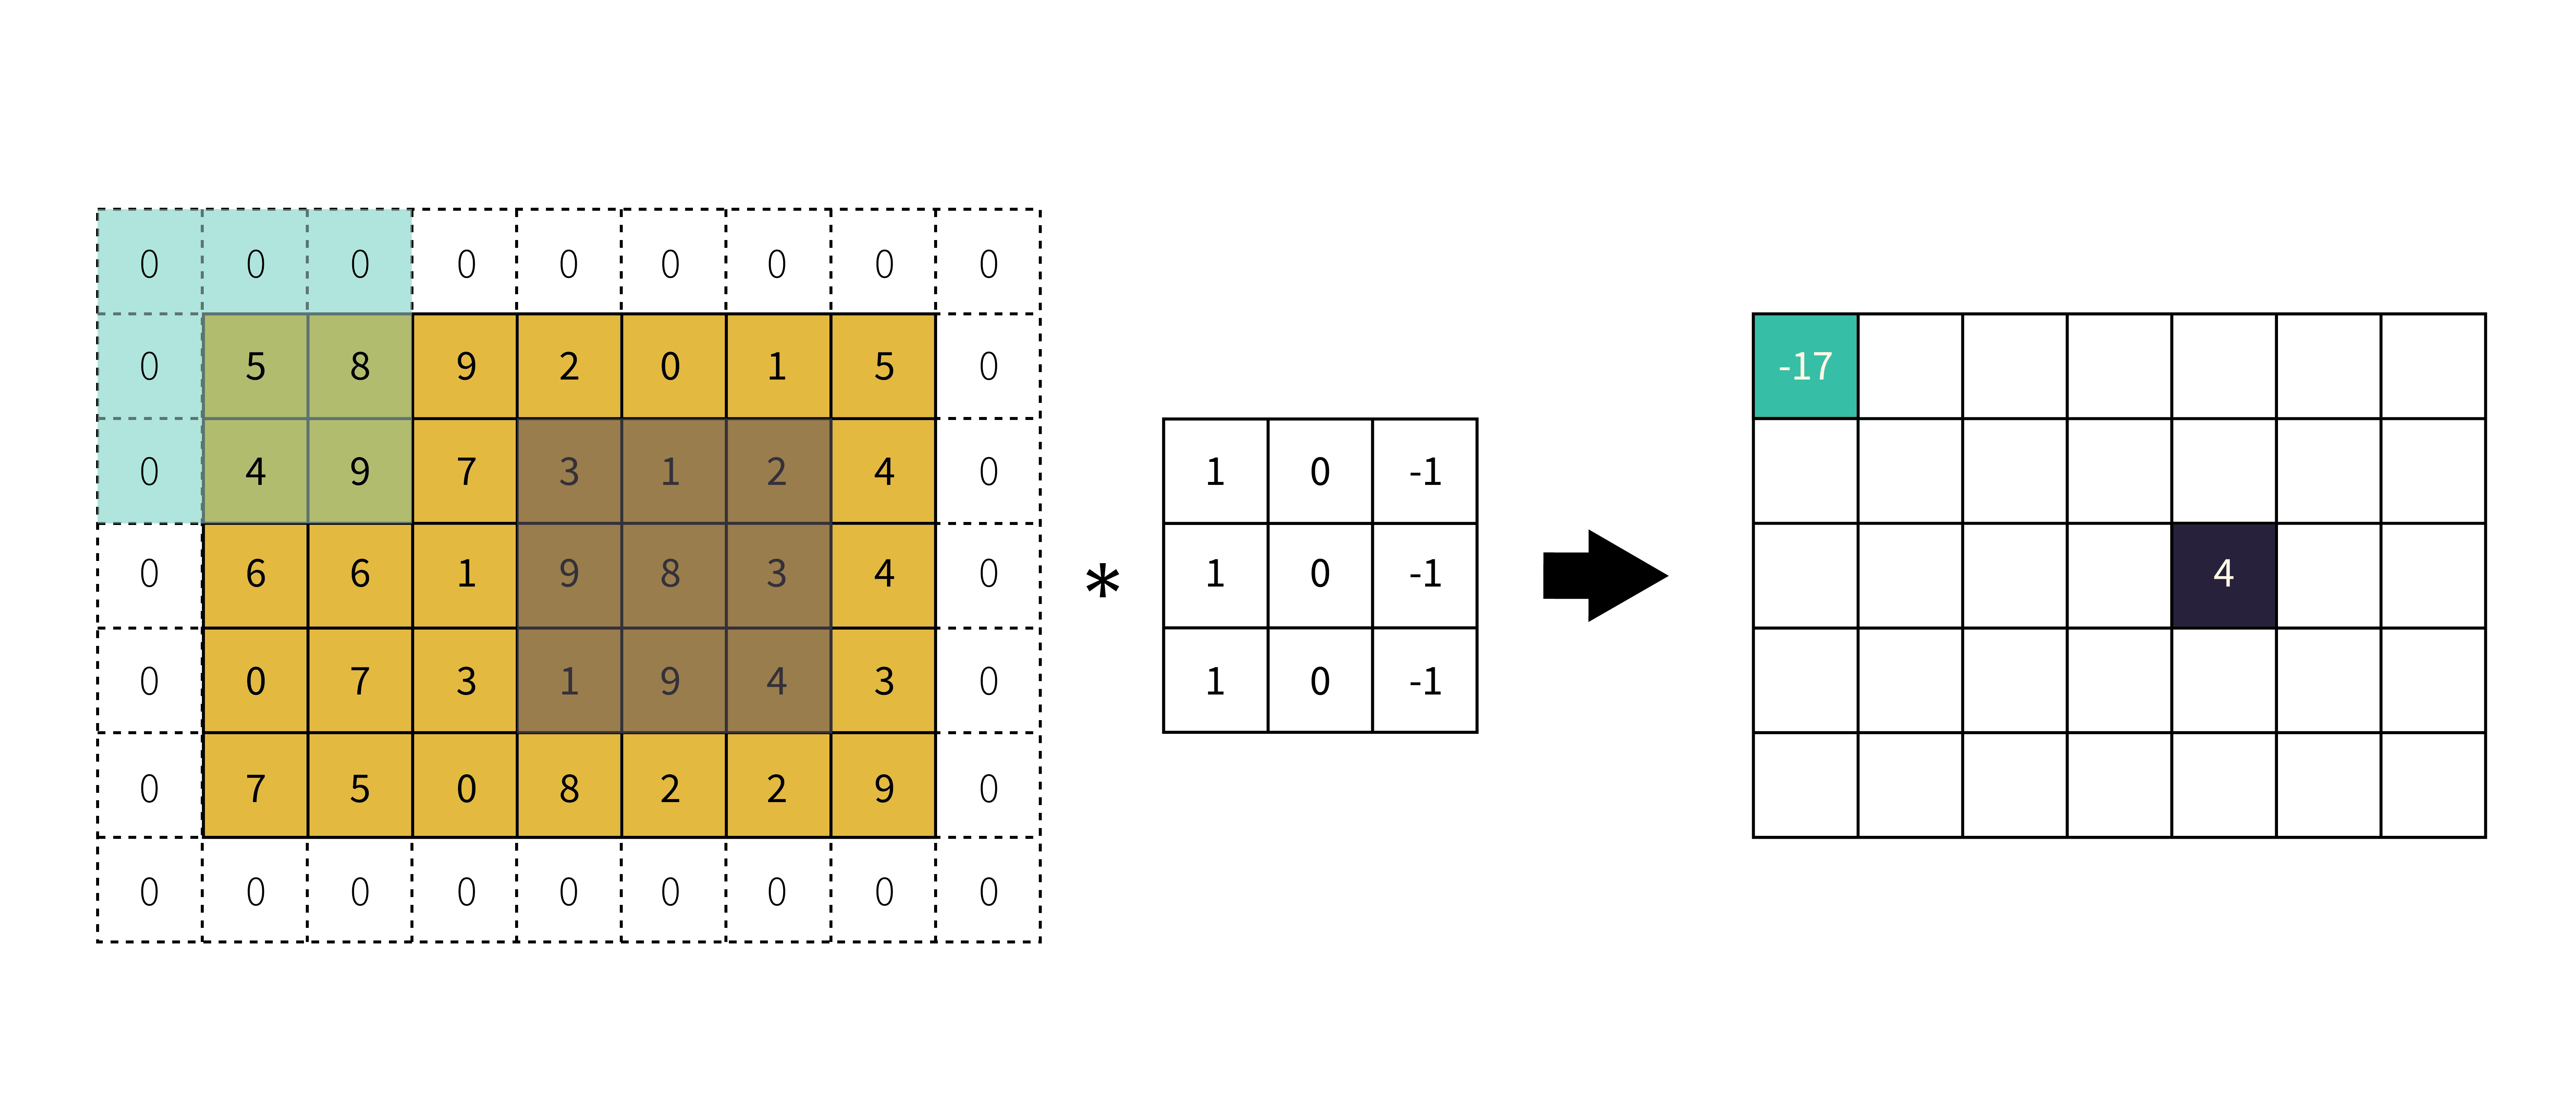
\includegraphics[width = 5in]{../cap2_CNNs/src/padding.png}
     \caption{\textcolor{red}{Usar una imagen propia}}
 \end{figure} 
 Para solucionar este problema, en vez de hacer la convolución con la imagen original $I$, extendemos la imagen hacia todos lados $\frac{k-1}{2}$ pixeles y realizamos una nueva convolución con la imagen extendida $\tilde I$.
 La nueva imagen $\tilde I$ contiene la misma información que la imagen original $I$, por tanto no importa la información que se añada en los nuevos pixeles. Sin embargo varias estrategias heurísticas han sido desarrolladas con el paso de los años:
\begin{itemize}
    \item \textcolor{red}{\textbf{Constant Padding.}} Cuando  se agrega un valor $c$ en todo el borde. Cuando $c = 0$ se conoce como \textcolor{red}{Zero Padding}.
    \item \textcolor{red}{\textbf{Zero Padding.}} Una posible opción y de las más utilizadas, es agregar ceros en el borde. En \cite{padding} se descubrió que utilizando este tipo de \textcolor{red}{padding} codifica cierto grado de información de las posiciones absolutas. Efecto que no ocurre cuando no se utiliza ningún tipo de \textcolor{red}{padding}. 
    \item \textcolor{red}{\textbf{Reflection Padding.}} Este padding se basa en reflejar los valores con respecto al borde \cite{type_of_paddings}.
    \item \textcolor{red}{\textbf{Symmetric Padding.}} Este padding es muy similar al \textcolor{red}{reflection padding}. En cada fila toma todos los valores y los invierte. Siendo esto lo que aparece en los bordes.
\end{itemize}
\begin{definition}
    Sea $x\in \mathbb R^{h\times w}$ una característica. Sea $\tilde x \in R^{(h+2s)\times (w+2r)}$ con $s < h$ y $r < w$ la característica extendida. Definimos algunos de los \textcolor{red}{paddings} como sigue: 
    \begin{enumerate}
        \item \textcolor{red}{Zero Padding}: 
        \begin{equation}           
            \tilde x_{i,j} = \left\{ 
                \begin{matrix}
                    x_{i-s, j-r} & \text{si} & s< i <h+s \quad \text{ y } \quad r< j < w+r \\
                    0 & \text{en otro caso}
                \end{matrix}
            \right..
        \end{equation}
        \item \textcolor{red}{Reflection Padding}:
        \begin{equation}           
            \tilde x_{i,j} = \left\{ 
                \begin{matrix}
                    x_{i-s, j-r} & \text{si} & s< i <h+s \quad \text{ y } \quad r< j < w+r \\
                    x_{i-s, r-j+2} & \text{si} & j < r \\
                    x_{s-i+2, j-r} & \text{si} & i < s \\
                    x_{2h+s-i, j-r} & \text{si} & i > h+s \\
                    x_{i-s, 2w+r-j} & \text{si} & j > w+r \\
                \end{matrix}
            \right..
        \end{equation}
    \end{enumerate}  
\end{definition}
En \cite{type_of_paddings} tras un estudio exhaustivo en el Image Net concluyen que el \textcolor{red}{symmetric padding} y el \textcolor{red}{reflection padding} obtienen peores resultados que el \textcolor{red}{Zero padding}. 
 %------------------------------ Pooling -----------------------
\subsection{Agrupación (Pooling)}
Una vez que la red encuentra características en una imagen, es posible que algunas secciones relevantes sean más grandes que otras. Por eso mismo, se implementa el \textcolor{red}{Downsampling}, es decir reducir el tamaño de las imágenes, para que nuestro kernel pueda encontrar cosas de distintos tamaños conforme las capas van reduciendo el tamaño de la imagen. La pregunta que surge es, ¿Cómo reducimos el tamaño de una imagen?  Sea como sea, siempre algo de información se pierde. Sin embargo existen métodos para resumir la información de varios pixeles en un sólo pixel. Algunos de estos métodos son
\begin{itemize}
    \item \textcolor{red}{\textbf{Max pooling}}. Dada una vecindad rectangular de pixeles, la \textcolor{red}{Max pooling} consiste en tomar el máximo valor dentro de esta vecindad. 
    \item \textcolor{red}{\textbf{Average pooling}}. Al igual que en el anterior caso, se toma una vecindad rectangular de pixeles. Sin embargo, en este caso se toma el promedio de todos los pixeles.
    \item \textbf{Un punto intermedio}. Considérese $v$ el vector de pixeles que debe reducirse a un sólo pixel . En \cite{pooling_analysis} se analiza el uso de diferentes agrupaciones, y se obtienen distintas parametrizaciones para hallar el valor del pixel $f_P(v)$ que sintetiza la información de $v$. Una posible parametrización es $f_P(v) = \left(\frac{1}{d}\sum_{i= 1}^{d}v_i^P\right)^{\frac{1}{P}}$. Donde $P=1$ es el \textcolor{red}{average pooling} y si $P\to \infty$ es el \textcolor{red}{max pooling}. Por tanto, es posible utilizar otros valores de $P$ para obtener \textcolor{red}{poolings} diferentes.
\end{itemize} 
\begin{figure}[H]
    \centering
    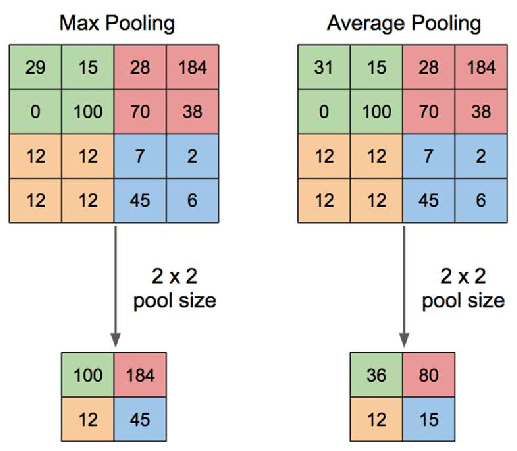
\includegraphics[width=4in]{../cap2_CNNs/src/pooling.png}
    \caption{\textsc{Ejemplo de maxpooling y averagepooling con regiones rectangulares de $2\times 2$.}} 
\end{figure}
También es posible en vez de hacer un \textcolor{red}{pooling} hacer una convolución con cierto tamaño de paso, con la intención de reducir el tamaño de la imagen. Esto no ha remplazado al \textcolor{red}{maxpooling} pero en la literatura se observan resultados prometedores. 
% ------------------------ Global pooling layers
\subsubsection{\textcolor{red}{Global pooling layers} }
Además de hacer un \textcolor{red}{downsampling}, también es común que en algún punto de la red, se reduzca una característica a un valor escalar, o en caso de una imagen con $d$ canales es posible obtener un vector en $\mathbb R^d$ \cite{CNNdefinition}.
\begin{definition}
    Sea $x\in \mathbb R^{h\times w}$ una característica. El operador \textcolor{red}{global average pooling}, $P_g: \mathbb R^{hw}\to \mathbb R$ se define como:
    \begin{equation}
        P_g(x) = \frac{1}{hw}\sum_{i=1}^h\sum_{j=1}^w x_{i,j}.
    \end{equation}
    Más aún, sea $x \in \mathbb R^{h\times w \times d}$ una característica. El operador \textcolor{red}{global average pooling}, $P_g: \mathbb R^{hw}\to \mathbb R$ se define como:
    \begin{equation}
        P_g(x) = (P_g(x_1), ..., P_g(x_d)).
    \end{equation}
\end{definition}
% ------------------------ Convolución como una operación lineal
\subsection{Convolución como una operación lineal}
 Es posible ver una convolución como una multiplicación por una matriz poco densa, en donde varios elementos de la matriz están restringidos a ser iguales a otros. Para las convoluciones de una variable, tiene que ser una \textsl{matriz de toeplitz}. En lo que refiere a dos dimensiones, una convolución es equivalente a una \textsl{Doble Matriz Circulante por Bloques} [Definición \ref{doubly_circulant_matrix}]. Es decir, se tiene lo siguiente 
 \begin{corollary}
    Sea $I$ una imagen, y $K$ un kernel. Existe una matriz $\hat K$ 
    \begin{equation}
        I*K = \text{vec}(I)\hat K.
    \end{equation}
 \end{corollary}

 %------------------------------ Redes Neuronales convolucionales -----------------------
\section{Redes Neuronales Convolucionales}
\label{section_cnn}
Consideremos el problema de clasificación. Sea $m$ la cantidad de clases posibles. Dados $y_1, y_2, ..., y_s \in \mathbb R^d$ y sus etiquetas $c_1, c_2, ..., c_s\in \mathbb R^m$, en donde la $k$-ésima entrada de $c_i$ puede ser $1$ o $0$. Cada vector $c_i$ tiene únicamente una entrada con valor $1$, que determina exactamente a que clase pertenece $y_i$.

    Sean 
    \begin{equation}
        \label{clasification}
        Y_0 = [y_1, y_2, ..., y_s]^T \quad \text{ y }, \quad  C = [c_1, ..., c_s]^T.
    \end{equation}

    El objetivo es poder clasificar correctamente datos no etiquetados. Para ello se han desarrollado diferentes arquitecturas de redes neuronales, y en el 2015 las Redes Neuronales Convolucionales obtuvieron el primer lugar en el concurso Image Net \cite{imageNet_dataset}, consiguiendo resultados sin precedenes \cite{resnet0}. 


 %------------- Descenso del gradiente
\subsection{Descenso del Gradiente Estocástico}
Ya que el problema de aprendizaje, es un problema de optimización, podemos recurrir a la teoría de optimización conocida. El algoritmo más común en el aprendizaje automático es el \textsl{descenso de gradiente estocástico} (SGD por sus siglas en inglés), el cuál es un algoritmo numérico para encontrar mínimos locales de una función. La intuición se basa en que si se tiene un punto $x\in D_f$, la dirección en dónde más decrece es $-\nabla f$. Éste método consiste en dos pasos
\begin{enumerate}
    \item Se selecciona un punto inicial $x_0$ en el dominio.
    \item Se actualiza nuestro valor $x_{i+1} = x_i - \alpha\nabla f(x_i)$ para $i = 1, ... N$
\end{enumerate}
donde $N$ es el número de iteraciones totales y $\alpha$ es un escalar, el cuál se conoce como razón de aprendizaje (learning rate). Es importante seleccionar una razón de aprendizaje apropiado, pues en caso de seleccionar una muy grande, el algoritmo podría diverger, por el contrario si se selecciona una muy pequeño, entonces el entrenamiento podría ser demasiado lento. 

Para calcular el gradiente de manera exacta, es necesario utilizar todo el conjunto de datos, lo cuál puede traducirse a tiempos elevados de cómputo. Es por eso, que en la práctica, se utiliza únicamente un subconjunto aleatorio de datos, calculando así, una aproximación al gradiente $\nabla J$ de la funcion de costo. Debido a este artificio que reduce el tiempo de entrenamiento, es que nuestro algoritmo es considerado estocástico.
\begin{figure}[H]
    \centering
    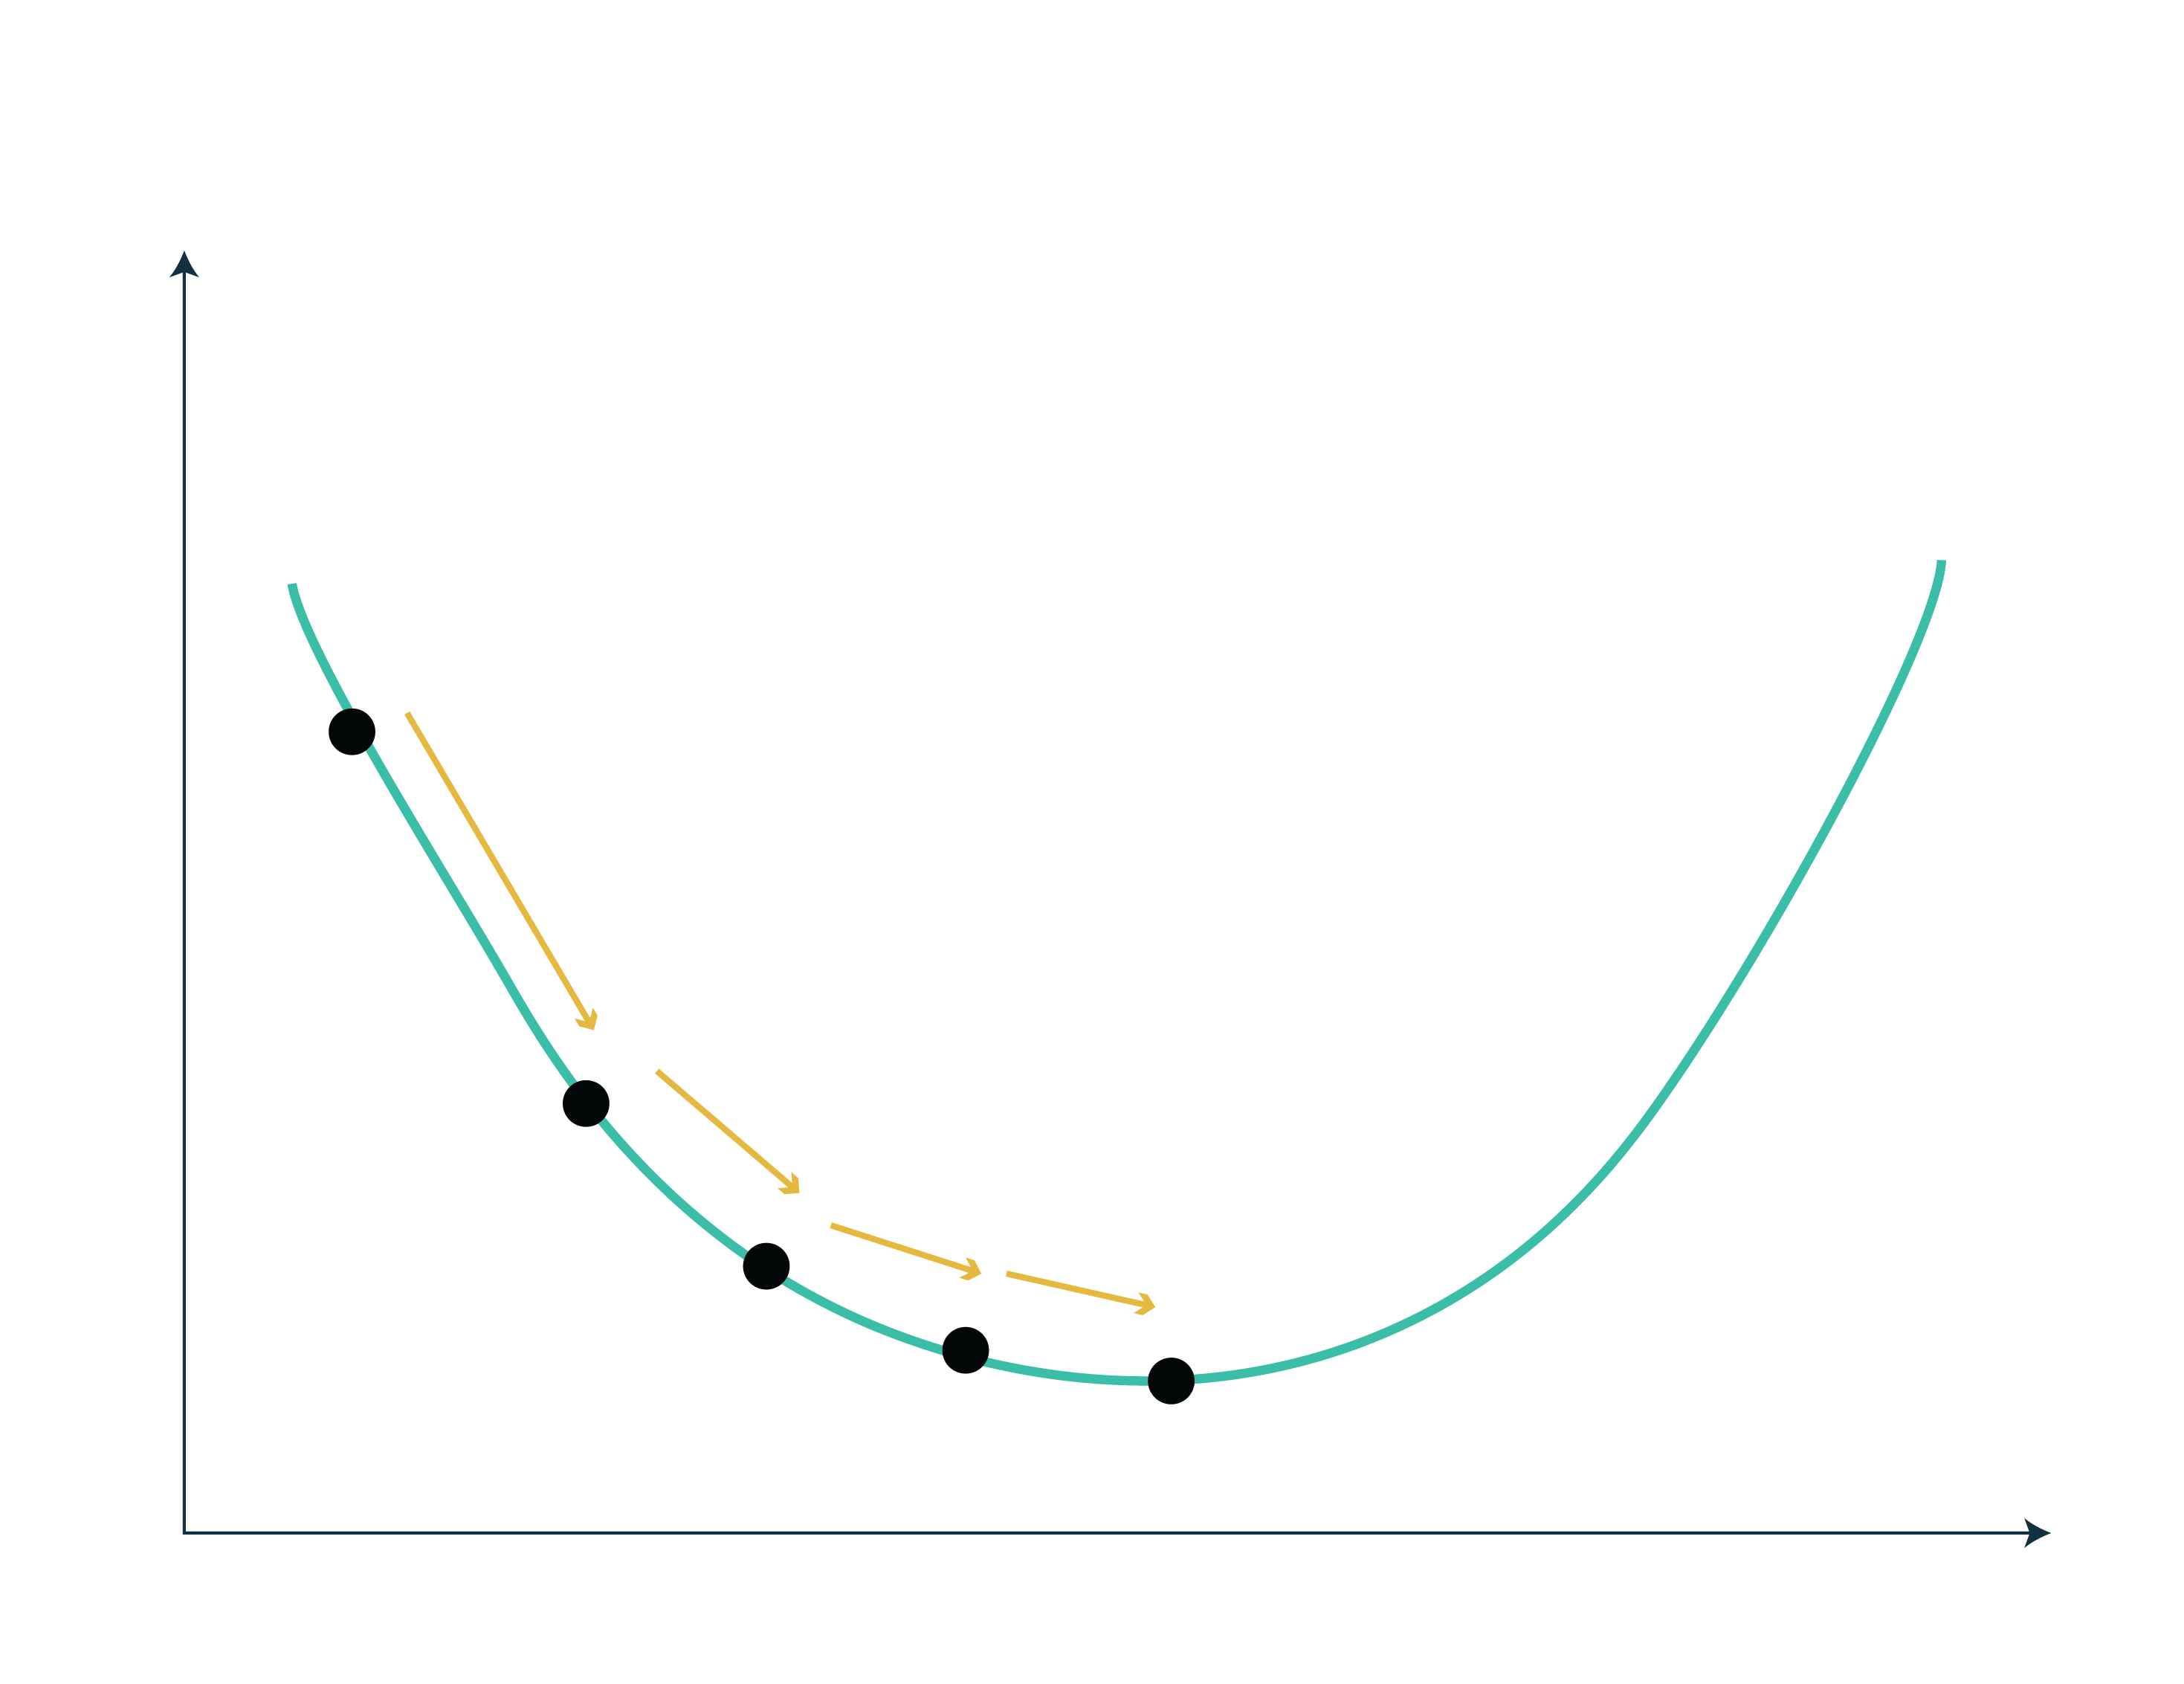
\includegraphics[width=4in]{../cap2_CNNs/src/sgd.png}
    \caption{\textcolor{red}{Seleccionar su propia imagen}} 
\end{figure}
\subsection{Optimizadores}
\label{subsection:optimizadores}
Existe una amplia literatura en el área de optimización de funciones. Por lo que es natural pensar que el SGD no es el único método para optimizar la función de costo. Debido a que la evaluación de dicha función, involucra millones de parámetros en las redes profundas actuales, no todos los algoritmos de optimización son adecuados para esta tarea. Aquí se presentan los métodos más efectivos investigados en los últimos años.

\subsubsection{AdaGrad}
A diferencia del SGD, el Algoritmo de Gradiente Adaptativo o AdaGrad \cite{adagrad}, actualiza la razón de aprendizaje con cada iteración. El algoritmo tiene un mejor desempeño en presencia de gradientes dispersos, es decir cuando el vector del gradiente contiene varios ceros.

\begin{equation}
    \theta_t = \theta_{t-1} - \frac{\alpha}{\sqrt{b_t} + \epsilon} g_{t-1}
\end{equation}
dónde $b_{t-1}$ es la suma del cuadrado de los gradientes.
\begin{equation}
    b_t = \sum_{i=1}^tg_{t-1}^2
\end{equation}

\subsubsection{RMSProp}
El algoritmo RMSProp fue propuesto por Geoff Hinton motivado en resolver el problema de las razones de aprendizaje sumamente pequeñas que se obtenían con el algoritmo AdaGrad y por consiguiente, evitar el desvanecimiento del gradiente.

\begin{equation}
    E[g^2]_t = \beta E[g^2]_{t-1} + (1-\beta)g_t^2
\end{equation}
\begin{equation}
    \theta_t = \theta_{t-1} - \frac{\alpha}{\sqrt{E[g^2]_t + \epsilon}}g_t
\end{equation}
\subsubsection{Adam}
El Estimador de momento Adaptativo (Adam por sus siglas en inglés) \cite{adam} se basa en momentos de primer y segundo orden del gradiente. Este método fue creado con la intención de obtener los beneficios de 2 optimizadores anteriores: el AdaGrad y el RMSProp. 


Para calcular los parámetros $\theta_t$, es necesario calcular el gradiente $g_t= \nabla f(\theta_{t-1})$. Denotamos  $m_t$ a la media movil exponencial, y $v_t$ al gradiente cuadrado. Los cuales se calculan de la siguiente manera:
\begin{equation}
    m_t = \beta_1 m_{t-1} + (1-\beta_1)g_t,
\end{equation}
\begin{equation}
    g_t = \beta_2 v_{t-1} + (1-\beta_2)g_t^2,
\end{equation}
dónde $\beta_1, \beta_2\in [0,1)$ son hiperparámetros que controlan el decrecimiento exponencial.

Los momentos $\hat m_t$ y $\hat v_t$ son la media y la varianza no centrada respectivamente.

\begin{equation}
    \hat m_t = \frac{m_t }{1-\beta_1^t},
\end{equation}
\begin{equation}
    \hat v_t = \frac{v_t}{1-\beta_2^t}.
\end{equation}

El optimizador Adam, actualiza los parámetros de la siguiente manera:
\begin{equation}
    \theta_t = \theta_{t-1} - \frac{\alpha \hat m_t}{\sqrt{\hat v_t} + \epsilon}.
\end{equation}
Dónde $\alpha$ es el tamaño de paso y $\epsilon$ es un valor cercano a cero.
\subsection{Propagación hacia atrás}
Ahora que se tiene un algoritmo para optimizar una función de costo, la pregunta natural es ¿Cómo obtenemos el gradiente? Siendo la propagación hacia adelante de una red, una función tan complicada y con tantos parámetros, es muy difícil calcular de manera analítica nuestro gradiente. Por buena suerte para nosotros, existe una técnica conocida como \textsl{propagación hacia atrás}, encargada de calcular numéricamente el gradiente de la función de costo.


\subsection{Normalización por Lotes}
Entre las téncicas de regularización más utilizadas se encuentra la \textsl{normalización por lotes} (BN por sus siglas en inglés). En el 2015 en un artículo de google \cite{batchNormalization} se describe esta técnica y se constata que tiene múltiples beneficios tales como incrementar la razón de aprendizaje, conseguir que el entrenamiento sea más independiente de la inicialización y además actuar como regularizador.

\begin{definition}
    Sea $\mathcal{B} = \{x^{(1)}, x^{(2)}, \ddots, x^{(m)}\}$ un lote de características. La normalización por lotes de $\mathcal B$ se define como:
    \begin{equation}
        B(x^{(i)}; \gamma, \beta) := \frac{\gamma(x^{(i) - \mu})}{\sigma} + \beta, \quad i=1,2...,m,
    \end{equation}
    donde  $\mu := \sum^m_{i=1}x^{(i)}/m$ y $\sigma^2 = \sum^m_{i=1}(x^{(i)}-\mu)^2/m$.
\end{definition}
Los parámetros $\gamma$ y $\beta$ usualmente se aprenden en la optimización. Cuando se usa la normalización por lotes, no es necesario agregar \textcolor{red}{biases} pues son calculados explícitamente a través de $\beta$.

Ahora que conocemos lo que es una convolución, se define matemáticamente una Red Neuronal Convolucional.   
\begin{definition} 
    Sea $x_0\in \mathbb R^{h\times w\times d}$ una característica. La propagación hacia adelante de una CNN está determinada por el siguiente esquema recursivo

    \begin{equation}
        x_{n+1} = \sigma(x_n * K_n + b_n).
    \end{equation}
    donde $\sigma$ es una función de activación, $K_n$ representa un Kernel y $b_n\in \mathbb R^d$ es el \textcolor{blue}{bias}.
\end{definition}
En las primeras arquitecturas sea usaban Redes Completamente Conectadas (FCN por sus siglas en inglés) tal como se aprecia en la Figura \ref{cnn_example_img}. Sin embargo en los últimos años se ha visto un incremento en el uso de Redes Completamente Convolucionales.

\begin{figure}[H]
    \centering
    
    \includegraphics[width=5in]{../cap2_CNNs/src/convolution_arquitecture.png}
    \caption{\label{cnn_example_img} Ejemplo de arquitectura de una Red Neuronal Convolucional. En la figura se aprecia la imagen de entrada, las capas convolucionales y la FCN que determina la clase \cite{image:cnn}} 

\end{figure}


\subsection{Desvanecimiento del gradiente}
Los mayoría de los algoritmos de optimización, dependen del gradiente. Y los algoritmos que utilizan la propagación hacia atrás, en ocasiones presentan el problema conocido como \textsl{desvanecimiento del gradiente}, que consiste en que los gradientes se vuelven tan pequeños que previenen al modelo de continuar con el proceso de aprendizaje.

\subsection{CNNs en el Estado del Arte}
En 2012 en el ImageNet ocurrió algo sin precedentes en dicha competencia. El ganador del concurso se había llevado el primer lugar absoluto, obteniendo una ventaja de 10.9$\%$ de error por debajo del segundo lugar. Es así como la \textsl{AlexNet} \cite{alexnet} consiguió reputación para las CNNs. Para 2013, la red ganadora del ImageNet(2013) fue la Zf-net \cite{zfnet}, la cuál era una modificación de los hiperparámetros de la AlexNet.

\begin{figure}[H]
    \centering
    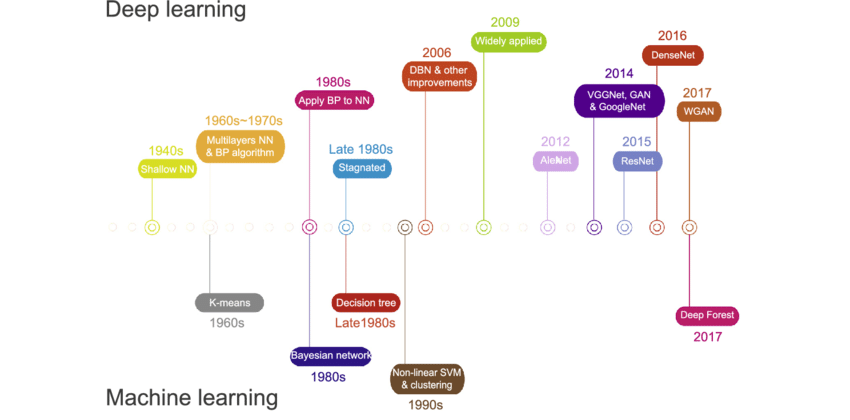
\includegraphics[width=5in]{../cap2_CNNs/src/timeline.png}
    \caption{Línea de tiempo de las Redes en el Estado del Arte} 
\end{figure}
 %------------------------------ ResNet -----------------------
\section{ResNet}
\label{resnet_section}
Las \textsl{Redes Neuronales Residuales} fueron presentadas en 2015 por Kaiming He et. al. en \cite{resnet0}. Uno de los mayores retos en el diseño de redes profundas, es el \textsl{desvanecimiento del gradiente}. Es decir, por la naturaleza de la propagación hacia atrás, las redes muy profundas, implican el cálculo de gradientes con entradas muy pequeñas, y eventualmente el gradiente se desvanece y previende el aprendizaje de la red.
Es decir, $\|\nabla_\theta L\| = 0$ dónde $L$ es la función de pérdida y $\theta$ son los parámetros. 

Antes del 2015 existían dificultades para alcanzar redes con profundidades mayores a 20 capas. Para solucionar este problema, se crearon las \textsl{conexiones de salto}.

\begin{definition} 
    Consideremos el problema de clasificación (\ref{clasification}). Sea $x_0\in \mathbb R^h\times w\times d$ una característica. La propagación hacia adelante de la ResNet está determinada por el siguiente esquema recursivo 

    \begin{equation}
        \label{resnet_equation}
        x_{n+1} = x_n + \sigma(x_n * K_n + b_n).
    \end{equation}
    donde $\sigma$ es una función de activación, $K_n$ representa un Kernel y $b_n\in \mathbb R^d$ es el \textcolor{blue}{bias}.
\end{definition}
Ya que la operación de convolución puede ser expresada como una multiplicación de matrices, es posible reescribir la ecuación (\ref{resnet_equation}) como:
\begin{equation}
    \label{resnet_equation_modified}
    X_{n+1} = X_n + \sigma(X_nA_n + b_n).
\end{equation}
dónde $X_0 = \vect{x_0}$ y $A_n$ es la matriz que induce el kernel $K_n$. 

La diferencia entre una CNN convencional es el término $X_n$ que se agrega a $\sigma(\cdot)$, conocida como conexión de salto, cuyo propósito es estabilizar el gradiente, para evitar su explosión o desvanecimiento.

\begin{figure}[H]
    \centering
    
    \includegraphics[height=3in]{../cap2_CNNs/src/resnet_block.png}
    \caption{Diagrama de un bloque de ResNnet.} 

\end{figure}

Pese a que la ecuación (\ref{resnet_equation_modified}) es la forma canónica de definir una ResNet, también es posible usar otras funciones en vez de sólo la composición de la función de activación con una función lineal. Por lo que una definición más general de la ResNet es
\begin{equation}
    X_{n+1} = X_n + F_n(X_n) 
\end{equation}

En la ResNet original se observa que $F_n(x) = \sigma(xA_n + b_n)$. Sin embargo se han usado otras funciones. En \cite{DBLP:journals/corr/abs-1806-03751} se toma 
\begin{equation}
    \label{resnet_block_function}
    F_n(x) = \text{BN}(\hat K_n *\text{ReLU}(\text{BN}(K_n * x)))
\end{equation}
que en la versión de multiplicación de matrices es:
\begin{equation}
    F_n(x) = \text{BN}(\text{ReLU}(\text{BN}(x \cdot A_n)) \cdot B_n),
\end{equation}
dónde $A_n$ y $B_n$ son las matrices correspondientes a los filtros $K_n$ y $\hat K_n$ de manera respectiva, BN y ReLU son las funciones de Normalización por lotes y Unión lineal Rectificada y la operación $M\cdot N$ es la multiplicación de matrices convencional colocada para mayor claridad.  

La función (\ref{resnet_block_function}) es también la utilizada en la biblioteca de pyTorch \cite{pytorch_library} en el repositorio:\\
\\
\url{https://github.com/pytorch/vision/blob/main/torchvision/models/resnet.py}. \\
\\
Además de los bloques con conexiones de salto, las arquitecturas modernas cuentan con otras capas, incluyendo capas convolucionales, normalizaciones e incluso una Red Completamente Conectada (FCN por sus siglas en inglés) en la parte final de la propagación. Una de las ResNet más populares, es la ResNet-50


\begin{figure}[H]
    \centering
    \includegraphics[width=4in]{../cap2_CNNs/src/resnet50.png}
    \caption{Diagrama de una ResNet-50} 
\end{figure}
%------------- Estabilidad de las redes neuronales
\subsection{Inicialización de parámetros}
Los algoritmos de optimización (Sección \ref{subsection:optimizadores}) requieren de un valor inicial $\theta_0$. En la mayoría de los casos, una selección adecuada de $\theta_0$ puede conseguir que el número de iteraciones se reduzca en comparación con un $\theta_0$ arbitrario. El Artículo \cite{weight_initialization} contiene un análisis dedicado a la inicialización de parámetros para aprendizaje profundo.

\subsubsection{Inicialización con Ceros}
Inicializar los parámetros con ceros es un acercamiento natural. Sin embargo, es conocido que si dos parámetros con la misma función de activación, están conectados con la misma entrada, entonces se modificarán de igual forma en el proceso de entrenamiento. De modo que se dice que la inicialización deber \textsl{romper la simetría} \cite{deeplearningbook}. El caso de la inicialización con ceros, o con cualquier constante, no satisface esta propiedad, por lo que no es recomendable usarlas.
\subsubsection{Inicialización Aleatoria}
Una manera sencilla de romper la simetría es  inicializando los parámetros de manera aleatoria. Una heurística común es inicializar la matriz de pesos $W$ con una distribución uniforme
\begin{equation}
    W_{i,j} = U\left(-\frac{1}{\sqrt{m}}, \frac{1}{\sqrt{m}}\right),
\end{equation}
donde $m$ es la cantidad de entradas, y $U[-a,a]$ la distribución uniforme de $-a$ hasta $a$. Sin embargo, al no prestar atención al comportamiento de los gradientes, esta forma de inicializar nuestros parámetros puede provocar desvanecimiento o  explosión del gradiente.
\subsubsection{Inicialización de Glorot}
Para \textsl{Inicialización de Glorot}, también conocida como la \textsl{inicialización de Xavier} \cite{glorot_initialization} se asume que los pesos son inicializados independientemente y que las varianzas de las características de entrada son iguales. Además se pretende que las varianzas de los gradientes en todas las capas sean iguales. Para ello se propone la siguiente inicialización :
\begin{equation}
    W_{i,j} \sim U\left(-\sqrt{\frac{6}{m+n}}, \sqrt{\frac{6}{m+n}}\right)
\end{equation}
donde se tienen $m$ valores de entrada y $n$ valores de salida.

\subsubsection{Inicialización con Kaiming}
La \textsl{inicialización de Kaiming} o \textsl{Inicialización de He} \cite{kaiming} asume funciones de activación del tipo Rectificador, tales como la ReLu o la PReLU. 
\begin{equation}
    W_l \sim \mathcal{N} \left(0, \frac{2}{n^l}  \right)
\end{equation}
dónde $n_l$ es la cantidad de elementos en la capa l.

 %------------- Estabilidad de las redes neuronales
\subsection{Estabilidad en las redes Neuronales}
\label{resnet_stability_introduction}
En clasificación de imágenes, una red debe ser robusta contra el ruido, o pequeñas modificaciones en la imagen.  En el artículo \cite{CNNdefinition} se establecen definiciones formales de estabilidad, cuyo principio básico es que la salida debe ser continua con respecto a la entrada.

\begin{definition}
    Supóngase $f$ la propagación hacia adelante de una red neuronal. Sea $x$ una imagen y $\hat x$ la misma imagen perturbada. Decimos que $f$ es estable con respecto a epsilon cuando 
    \begin{equation}
        \|f(x)-f(\hat x)\| < \epsilon
    \end{equation}
\end{definition}
En la práctica se pretende reducir lo más posible el valor de $\epsilon$. En \cite{stable_resnets} se agrega un término $h\in \mathbb R$ a la ResNet con la intención de añadirle estabilidad a la red
\begin{equation}
    X_{n+1} = X_n + h\sigma(X_nA_n + b_n).
\end{equation}
%%%%%%%%%%%%%%%%%%%%%%%% CHAPTER 1%%%%%%%%%%%%%%%%%%%%%%%%%%%%%%%%


\chapter{Ecuaciones diferenciales}
\label{odes_chapter}
Las ResNets y las Ecuaciones Diferenciales Ordinarias guardan cierta relación que será estudiada a detalle en el Capítulo \ref{odes_and_resnets}. En este capítulo se presenta una introducción a las Ecuaciones Diferenciales Ordinarias (ODEs por sus siglas en inglés) y a los métodos numéricos necesarios para su resolusión. Para un estudio más extensivo se puede consultar \cite{sauer, Ascher}.

Desde su implementación en el sigo XVII \cite{ode_history} las ecuaciones diferenciales han sido una herramienta de mucha utilidad para las ciencias, con aplicaciones en geometría \cite{geometry_and_odes}, mecánica \cite{classical_mechanics}, electromagnetismo \cite{electromagnetism_and_odes}, etc.

Una ecuación diferencial ordinaria se representa de la siguiente manera:
\begin{equation}
    \frac{dx}{dt} = f(x(t), t),
\end{equation}
donde $f: \mathbb R^m \to \mathbb R^n$.
En caso de que no exista ambiguedad, es posible escribir $x$ en lugar de $x(t)$ y $x'$ para referirse a la derivada de $x$ con respecto a $t$, con lo que la ecuación anterior se puede escribir de la siguiente manera:
\begin{equation}
    x' = f(x,t)
\end{equation}
En este caso, ya que la variable dependiente es el tiempo $t$, la derivada con respecto al tiempo se puede escribir con un punto, es decir: $\dot x = \frac{dx}{dt}$. En este trabajo, la variable dependiente será el tiempo, pero la teoría se puede extender para distintos dominios.
\section{Problemas de valor inicial}
Considérese el siguiente problema de valor inicial (IVP por sus siglas en inglés)
\begin{align}
    \label{ode} \dot x(t) = f(x, t),& \quad t>0\\
    \label{initial_value} x(t_0) = \nu,&
\end{align}
donde $t\in [t_0, t_f]$. 

\subsection{Existencia, unicidad y continuidad de soluciones}
\begin{theorem}
    Sea $f: [a_1,b_1] \times [a_2, b_2]$ una una función Lipschitz continua en la segunda entrada y $a_2 < x_a < b_2$. Entonces existe un $c\in [a_1, b_1]$ tal que el IVP
    \begin{equation}
        \left\{\quad \begin{matrix}
            \dot x = f(x,t) \\
            x(a_1) = x_a \\
            t \in [a_1,c]
        \end{matrix}\right.
    \end{equation} 
    tiene exactamente una solución $x(t)$. Aún más, si $f$ es Lipschitz continua en $[a_1, b_1]\times (-\infty, \infty)$, entonces existe exactamente una solución en $[a_1, b_1]$. 
\end{theorem}
La demostración se puede encontrar en \cite{sauer}

\section{Estabilidad}
\label{ode_stability}
En la literatura, no existe una convención al hablar de estabilidad de ecuaciones diferenciales \cite{richard-Bellman, Hyers-Ulam}, sin embargo adoptaremos las definiciones de Ascher \cite{ascher-book}.

Cuando se hacen cambios mínimos en el valor inicial del IVP (\ref{ode} - \ref{initial_value}), uno se pregunta ¿qué ocurre con la solución? ¿Los cambios también serán pequeños? Para el análisis de estabilidad esto, se requieren algunas definiciones

\begin{definition}
    Una solución $x(t)$ es llamada \textbf{estable} si para todo $\varepsilon > 0$ existe un $\delta > 0$ tal que cualquier otra solución $\hat x(t)$ de \ref{ode} que satisfaga 
    \begin{equation}
        |x(t_0)  - \hat x(t_0)| \leq \delta
    \end{equation}
    también satisface 
    \begin{equation}
        \label{stable-ode}
        |x(t)- \hat x(t)| \leq \varepsilon, \quad \forall t > t_0.
    \end{equation} 
    La solución $x(t)$ es \textbf{asintónticamente estable} si en adición a (\ref{stable-ode}) se cumple que 
    \begin{equation}
        |x(t)- \hat x(t)| \to 0, \quad si \quad t\to \infty.
    \end{equation}
    Por otro lado, $x(t)$ es \textbf{relativamente estable} si en vez de (\ref{stable-ode}) se satisface que 
    \begin{equation}
        |x(t)- \hat x(t)| \leq \varepsilon|x(t)|, \quad \forall t > t_0.
    \end{equation}
\end{definition}

\begin{definition}
    Una solución es llamada \textbf{uniformemente estable} si, para cada $\varepsilon > 0$, existe $\delta > 0$ tal que cualquier otra solución $\hat x(t)$ de (\ref{ode}) que satisfaga
    \begin{equation}
        |x(c) - \hat x(c)| \leq \delta
    \end{equation}
    para algún punto $c \geq t_0$, también se satisface que
    \begin{equation}
        |x(t) - \hat x(t)| \leq \varepsilon, \quad \forall t > c.
    \end{equation}
\end{definition}

La \textbf{estabilidad asintótica uniforme} y la \textbf{estabilidad relativa uniforme} se definen de manera análoga. Es evidente que la estabilidad uniforme, implica estabilidad.

\subsection{Problema Lineal}
Considérese el IVP homogéneo 
    \begin{equation}
        \label{hom_ivp}
        \dot x = A(t)x, \quad  t > t_0
    \end{equation}
    \begin{equation}
        \label{hom_init}
        x(t_0) = \alpha
    \end{equation}


\begin{theorem}
    La solución $y$ IVP (\ref{hom_ivp}- \ref{hom_init}) con $A$ constante es uniformemente estable si y sólo si todos los eigenvalores de $A$ statisfacen que $\text{Re}(\lambda) < 0$ o si $\text{Re}(\lambda) = 0$ con $\lambda$ simple. 
\end{theorem}

Sin embargo, $A(t)$ no tiene por qué ser constante. Para un caso más general, se tiene el siguiente teorema.
\begin{theorem}
    \label{lineal_ivp}
    La solución $y$ del IVP (\ref{hom_ivp}- \ref{hom_init}) es uniformemente estable si se cumplen las siguentes dos condiciones
    \begin{enumerate}
        \item La matriz $A$ es \textbf{estrictamente diagonalmente dominante}, es decir 
        \begin{equation}
            \sum_{j\neq i} |a_{i,j}| \leq (1-\delta)|a_{ii}|, \quad i = 1, \cdots, n
        \end{equation}
        \item Los elementos de la diagonal son menores que 0 
        \begin{equation}
            Re(a_{ii}) < 0, \quad i = 1, \cdots n
        \end{equation}
    \end{enumerate}
\end{theorem}

Además, como consecuencia del Teorema de Gershgorin se tiene que si se satisfacen las hipótesis del Teorema (\ref{lineal_ivp}) los eigenvalores cumplen que $Re(\lambda_i) < 0$. De modo que los eigenvalores de nuestra matriz $A$ son elementos suficientes para determinar la estabilidad de una ecuación diferencial.

\subsection{IVP no lineales (El caso general)} 
\label{no_lineal_ivp}
Para determinar la estabilidad de un IVP no lineal, se puede hacer uso de los resultados obtenidos en la Subsección anterior. El tema de interés en esta ocasión es la ecuación 
\begin{equation}
    \label{original_ode}
    \dot x = f(x,t)
\end{equation}
\begin{equation}
    x(t_0) = \alpha
\end{equation}
Sea $\hat x$ una solución de (\ref{original_ode}), con $\hat x(t_0)$ no muy lejano de $x(t_0)$. Expandiendo $f(x,t)$ utilizando su serie de Taylor, se obtiene que 
\begin{equation}
    \label{taylor_for_ivp}
    f(\hat x, t) = f(y,t) + J(x,t)(\hat x - x) + r(x,\hat x, t),
\end{equation}
donde $J$ es el jacobiano definido por
\begin{equation}
    J(x, t) := \frac{\partial f}{ \partial x}.
\end{equation}
y el término $r$ es el residuo. Si se ignora el residuo $r$ en (\ref{taylor_for_ivp}), y tomando $z = x - \hat x$ se obtiene
\begin{equation}
    \dot z = J(t)z
\end{equation}
Por lo que para determinar la estabilidad, es suficiente conocer los eigenvalores del Jacobiano $J$.

\section{Métodos de Runge-Kutta}
Es posible generalizar el método de Euler, evaluando la derivada multiples veces en un paso. Esta idea se le atribuye a Runge \cite{book:110336}. y en 1901 Kutta hizo contribuciones importantes al método, dando paso a métodos de orden 4 y el primer método de orden 5, denominados métodos de Runge-Kutta. A continuación se describen alguno de los métodos de Runge-Kutta más relevantes.
\subsection{Método de Euler}
\label{section:euler_method}
La manera más elemental para resolver el IVP (\ref{ode} - \ref{initial_value}) es con el método de Euler. 

Nótese que es posible particionar el intervalo $[t_0, t_f]$ en $N$ partes iguales, obteniendo así la sucesión 
$$t_0, t_0 + h, t_0 + 2h, ... , t_0 + Nh,$$
donde
$$h = \frac{t_f - t_0}{N}.$$
Se denotará $t_n = t_0 + nh$ y  $x_n = x(t_n)$. De modo que se tiene la siguiente sucesión:
\begin{equation}
    t_0 < t_1 < t_2 < \cdots < t_N = t_f.
\end{equation}
El siguiente paso, es aproximar los valores de $x_n$, y a estas aproximaciones les llamaremos $w_n$, teniendo en cuenta que $w_0 = x_0$. Para ello, se hará uso de la expansión de Taylor de $x(t + h)$.
\begin{equation}
    \label{taylor}
    x(t + h) = x(t) + h\dot x(t) + R_1(t),
\end{equation}
donde $R_1(t)$ es el residuo de la expansión de Taylor. Sustituyendo $\dot x(t) = f(t, x(t))$, obtenemos 
\begin{equation}
    x(t+h) = x(t) + hf(t,x(t)) + R_1(t).
\end{equation}
Sustituyendo $t = t_n$ con $i < N$ obtenemos que
\begin{equation}
    x(t_n + h) = x(t_n) + hf(t_n, x(t_n)) + R_1(t_n).
\end{equation}
Por lo tanto, substrayendo $R_1(t)$, es posible obtener una sucesión que aproxime a la solución $x(t)$:
\begin{equation}
    w_{n+1} = w_n + hf(t_n, w_n), \quad w_0 = x_0.
\end{equation} 

\subsubsection{Error de truncamiento local}
En general, el error de truncamiento local de un método numérico, es el error generado a partir de una iteración. Es decir:
\begin{equation}
    e_n = |w_n - z(t_n)|
\end{equation}
donde $z$ es la solución del problema 
\begin{equation}
    \left\{
    \begin{matrix}
        \dot x = f(x,t) \\
        x(t_n) = w_n \\
        t \in [t_n, t_{n+1}]
    \end{matrix}    
    \right.
\end{equation}

En el caso del método de Euler, es posible encontrar el error de truncamiento local. Asumiendo que en la identidad (\ref{taylor}), $x(t)$ es doblemente diferenciable en el intervalo $(t_0, t_f)$, ocurre que
\begin{equation}
    R_1(t) = \frac{1}{2!} h^2\dot x(\xi),  \quad \xi\in (t, t+h).
\end{equation}
\subsubsection{Error de truncamiento global}
El error de truncamiento global de un método numérico, es el error generado por multiples iteraciones. 
\begin{equation}
    g_n = |w_n - x_n|
\end{equation}

Para investigar el error global del método de Euler, asúmase una cota superior $mh^2$ para la norma del error de truncamiento local, es decir $e_n \leq mh^2$. Además se asume Lipschitz continuidad para $f$, cuya constante de Lipschitz es $L$.

Es posible acotar el error global, de la siguiente manera:
\begin{equation}
    \label{bound_global_error}
    g_n \leq \frac{Ch^k}{L}(e^{L(t_n-a)}-1)
\end{equation}
La demostración de (\ref{bound_global_error}) puede encontrarse en \cite{sauer}. En general, se comparan los distintos métodos numéricos basándose en el error, y los mejores métodos son aquellos cuyo \textbf{orden} es mayor:
\begin{definition}
    Se dice que un método es de orden $\rho$ cuando $|w_n - x_n| = \mathcal O(h^{\rho})$.
\end{definition}

\subsection{Método de Euler modificado}
El siguiente método, es un ejemplo de un método de Runge-Kuta, el cuál se usará para desarrollar las ideas tras los métodos generales.
\begin{align*}
    k_1 &= f(t_n, w_n),\\
    k_2 &= f(t_n + \tfrac{1}{2}h,w_n + \tfrac{1}{2}hk_1),\\
    w_{n+1} &= w_n + hk_2,\\
    t_{n+1} &= t_{n}+h.
\end{align*}
Este es un método de segundo orden. 
\subsection{Método general}
El método de Runge-Kutta general con $s$ etapas se puede definir usando $s^2 + 2s$ números
\begin{equation}
    a_{i,j}, \quad i,j = 1,2,..., s. \qquad b_i, c_i, \quad i= 1, 2, ..., s,
\end{equation}
usando el siguiente esquema

\begin{equation}
    w_{n+1} = w_n + h\sum_{i=1}^sb_ik_i.
\end{equation}
En donde la sucesión $\{k_i\}$ es calculada usando la función $f$:
\begin{equation}
    k_i = f\left(t_n + c_ih, w_n + h\sum_{i=1}^sa_{i,j}k_i\right), \quad i = 1, 2, ..., s.
\end{equation}
Es posible determinar si el método es explícito o implícito, basándose en la matriz $A = \{a_{i,j}\}$. En caso de que sea una matriz triangular inferior, con todos los elementos de la diagonal iguales a cero ($a_{i,j} = 0$ para $j = i, i+1, ...,s$) el esquema es explícito.


Las siguientes relaciones, son conocidas como condiciones de orden
\begin{equation}
    \sum_{i=1}^s b_i=1, \quad \sum_{i,j=1}^sb_ia_{i,j}=\frac{1}{2}, \quad \sum_{i,j,k=1}^sb_i a_{i,j} a_{j,k}=\frac{1}{6}, \quad  \sum_{i,j,k=1}^sb_ia_{i,j}a_{i,k}=\frac{1}{3}
\end{equation}
y aseguran esquemas de al menos orden 3.

\subsection{Runge Kutta de orden 4 (RK4)}
Uno de los métodos más conocidos es el de orden 4
\begin{equation}
    w_{n+1} = w_n + \frac{h}{6}(s_1 + 2s_2 + 2s_3 + s_4),
\end{equation}
donde 
\begin{align*}
    s_1 &= f(t_n, w_n) \\
    s_2 &= f\left(t_n +\frac{h}{2}, w_n+\frac{h}{2}s_1\right)\\
    s_3 &= f\left(t_n +\frac{h}{2}, w_n+\frac{h}{2}s_2\right)\\
    s_4 &= f\left(t_n + h, w_n+hs_3\right).
\end{align*}
La simplicidad de este método, hace que sea muy fácil de programar, y al ser de orden 4, se prefiere por sobre otos métodos como Euler, o el Trapezoide. Como se puede apreciar, RK4 es un método de orden 4 y además tiene 4 etapas (i.e. $s=4$). Sin embargo, no se conoce cuántas etapas son necesarias para esquemas de órdenes mayores a 8. 
\subsection{Métodos de Runge Kutta simplécticos}
Dentro de la categoría de métodos de Runge Kutta, existen los métodos simplécticos \cite{symplecticRK}. Se caracterizan por preservar \textsl{invariantes cuadráticas} \cite{Sanz-Serna1988-mk, Lasagni1988-ov}.
\begin{definition}
    Un esquema de Runge Kutta se dice simpléctico si satisface la relación 
    \begin{equation}
        b_ia_{i,j} + b_ja_{j,i} - b_ib_j = 0, \quad i,j=1, ..., s.
    \end{equation}
\end{definition}
\subsection{Métodos implícitos}
Los métodos numéricos analizados hasta este momento se conocen como métodos explícitos, debido a que es posible calcular $w_{n+1}$ conociendo el valor $w_n$. 
\subsubsection{Euler hacia atrás}
Una versión implícita de Euler se conoce como Euler hacia atrás. 
\begin{align}
    w_0  &= x_0 \\
    \label{backward_euler} w_{n+1} &= w_n + hf(t_{n+1}, w_{n+1})
\end{align}
Difiere del método de Euler tradicional en que la pendiente que se usa involucra $w_{n+1}$. De modo que en cada nueva iteración, es necesario resolver un sistema de ecuaciones, y por consiguiente el costo computacional se incrementa.

%%%%%%%%%%%%%%%%%%%%%%%%% CHAPTER 1%%%%%%%%%%%%%%%%%%%%%%%%%%%%%%%%

\chapter{Teoría de control óptimo}
    
Las ResNets guardan cierta relación con las Ecuaciones Diferenciales \cite{stable_resnets}. En el Capítulo \ref{odes_and_resnets} se estudia la conexión entre las DNNs y las ODEs. Debido a esto y a que el problema de aprendizaje implica optimizar una función, el problema es equivalente a encontrar un \textsl{control óptimo}   

A continuación, se desarrollarán algunos resultados de Teoría de control  óptimo con base en \cite{suresh}.  

Cuando se habla de sistemas, se hace referencia a un proceso que cambia de estado conforme pasa el tiempo. En este caso considérese un sistema dinámico definido en el intervalo $[0, T]$ como
\begin{equation}
    \label{ch2system}
    \dot x =f(x(t),t), \quad x(0) = x_0,  
\end{equation}
donde $x(t)$, conocida como la \textsl{variable de estado} puede representar la producción de alimento en un tiempo $t$, el dinero recaudado en un tiempo $t$, o en general el estado de un proceso en un tiempo $t$. En logística y física, existen variables que se pueden controlar, como la cantidad de publicidad, o la reinversión de capital cada cierto momento, con lo que es posible extender el sistema  (\ref{ch2system}) al siguiente:
\begin{equation}
    \label{ch2controlsystem}
    \dot x = f(x(t),u(t),t), \quad x(0) = x_0,
\end{equation}
donde la variable $u(t)$ es denominada \textsl{variable de control}. Conociendo la variable de control, es posible determinar la solución para $x$ en el sistema (\ref{ch2controlsystem}). El problema de control óptimo reside en maximizar la \textsl{función objetivo}, definida como
\begin{equation}
    J = \int_0^T F(x(t), u(t), t)dt + S[x(T), T].
\end{equation}
 La función $S$ determina el \textsl{valor de rescate} en el estado final $x(T)$ en el tiempo $T$, y obtiene pues en el área de economía es \textsl{el valor de un activo, una vez que ha concluido su vida útil} \cite{Engineerin_Economy}. Se denotará al conjunto de valores posibles de $u(t)$ como $\Omega(t)$.

\begin{definition}
    El \textsl{problema de control óptimo} es encontrar un valor admisible $u^*$ tal que 
    \begin{equation}
        \label{ch2umax}
        u^* = \max_{u(t)\in \Omega(t)}\left\{\int_0^T F(x, u, t)dt + S(x(T), T)\right\}
    \end{equation}
    con la condición 
    \begin{equation}
        \label{ch2dynamicCondition}
        \dot x = f(x,u,t), \quad x(0) = 0.
    \end{equation}
    La trayectoria óptima denotada como $x^*$ es la trayectoria que se obtiene cuando $u = u^*$.
\end{definition}

%Ecuación de Hamilton Jacobi Bellman
\section{La ecuación de Hamilton-Jacobi-Bellman}
Para estudiar la Ecuación de Hamilton-Jacobi-Bellman, es necesario el principio de optimalidad, el cuál establece que para obtener un camino óptimo de 0 a $T$, es necesario que para toda $t$, el camino de $t$ a $T$ sea óptimo también. Es importante remarcar que la siguiente prueba se encuentra en \cite{suresh} y se especifica que no tiene el propósito de ser rigurosa.

Sea $V: \R^n \times \R \to \R$ una función definida por
\begin{equation}
    \label{value_function}
    V(x,t) = \max_{u(s)\in \Omega(s)}\left\{\int_t^T F(x(s), u(s), s)ds + S(x(T), T)\right\}
\end{equation}
donde $s \geq t$.
Sea $\delta t$ un diminuto incremento en el tiempo, nótese que 
\begin{align*}
    V(x,t) - V(x(t + \delta t), t + \delta t) &= \max_{u(s)\in \Omega(s)}\left\{\int_t^T F(x(s), u(s), s)ds + S(x(T), T)\right\}  \\
    & \quad - \max_{u(s)\in \Omega(s)}\left\{\int_{t+ \delta}^T F(x(s), u(s), s)ds + S(x(T), T)\right\} \\
\end{align*}
Lo cuál, gracias al principio de optimalidad \cite{optimal_principle} se tiene que 
\begin{equation}
    \label{step_one}
   V(x(t), t) - V(x(t + \delta t), t + \delta t) = \max_{u(\tau)\in \Omega(\tau)} \left\{ \int_{t}^{t+ \delta t} F(x(\tau), u(\tau), \tau)\right\},
\end{equation} 
y por consiguiente
\begin{equation}
    \label{step_two}
    V(x(t), t) = \max_{u(\tau)\in \Omega(\tau)} \left\{ \int_{t}^{t+ \delta t} F(x(\tau), u(\tau), \tau) + V(x(t + \delta t), t + \delta t)\right\}.
 \end{equation} 
 Debido a que $F$ es una función continua, la integral en (\ref{step_two}) es igual a $F(x,u,t)\delta t$. Por consiguiente:
 \begin{equation}
    \label{2.11}
     V(x,t) = \max_{u\in \Omega(t)} F(x,u,t)\delta t + V[x(t+\delta t), t + \delta t] + \mathcal O(\delta t)
 \end{equation} 
 Asumiendo que la función $V$ es continuamente diferenciable en ambas entradas es posible hacer uso de la expansión de Taylor de $V$ en $\delta t$:
 \begin{equation}
    V[x(t + \delta t), t + \delta t] = V(x,t) + [V_x(x,t)\dot x + V_t(x,t)]\delta t + \mathcal O(\delta t)
 \end{equation}
 Sustituyendo (\ref{ch2controlsystem}) en (\ref{2.11}) se obtiene que 
 \begin{equation}
     V(x,t) = \max_{u\in \Omega(t)} \{F(x,u,t)\delta t + V(x,t) + V_x(x,t)f(x,u,t)\delta t + V_t(x,t)\delta t\} + \mathcal O(\delta t)
 \end{equation}
Cancelando $V(x,t)$ de ambos lados y dividiendo entre $\delta t$ se deduce que
\begin{equation}
    0 = \max_{u\in \Omega(t)} \{F(x,u,t) + V_x(x,t)f(x,u,t) + V_t(x,t)\} + \frac{\mathcal O(\delta t)}{\delta t},
\end{equation}
con lo que si $\delta t \to 0$ se tiene que 
\begin{equation}
    \label{pre_hamiltonian}
    0 = \max_{u\in \Omega(t)} \{F(x,u,t) + V_x(x,t)f(x,u,t) + V_t(x,t)\}
\end{equation}
dónde si se evalúa $t=T$ en $V$ se obtiene que 
\begin{equation}
    V(x,T) = S(x,T).
\end{equation}
Cuando la función $V$ es aplicada en el estado óptimo $x^*$ se obtiene un nuevo vetor
\begin{definition}(Vector de retorno marginal)
    Sea $V$ la función definida en (\ref{value_function}), el vector de retorno marginal $\lambda(t)$ se define como
    \begin{equation}
        \label{marginal_eq}
        \lambda(t) = V_x(x^*(t),t):=V_x(x,t)|_{x=x^*}
    \end{equation}
\end{definition}
Lo cuál será util para definir el concepto de Hamiltoniano.
\begin{definition}
    Considérese el sistema (\ref{ch2umax})-(\ref{ch2dynamicCondition}). Se denota el hamiltoniano $H: \R^n\times \R^m \times \R^n \times \R \to \R$ del sistema como 
    \begin{equation}
        \label{hamiltonian_def_eq}
        H(x,u,\lambda, t) = F(x,u,t) + \lambda f(x,u,t).
    \end{equation}
\end{definition}
La ecuación (\ref{pre_hamiltonian}) puede reescribirse como
\begin{equation}
    \max_{u\in \Omega(t)}[H(x,u,V_x,t) + V_t] = 0
\end{equation}
la cuál se conoce como \textsl{Ecuación de Hamilton-Jacobi-Bellman}(HJB). Más aún, ya que $V_t$ no depende de $u$ es posible retirar $V_t$ del operador $\max$.
\begin{equation}
    \label{HJB}
    \max_{u\in \Omega(t)}[H(x,u,V_x,t)] + V_t = 0.
\end{equation}
Gracias a la definición del control óptimo y de $\lambda(t)$, el operador $u^*$ maximiza la ecuación (\ref{HJB}), por tanto sea $u\in \Omega(t)$, se tiene que
\begin{equation}
    H[x^*(t), u^*(t), \lambda(t), t] + V_t(x^*(t),t ) \geq H[x^*(t), u(t), \lambda(t), t] + V_t(x^*(t),t )
\end{equation}
\begin{equation}
    \Rightarrow H[x^*(t), u^*(t), \lambda(t), t]  \geq H[x^*(t), u(t), \lambda(t), t].
\end{equation}

\section{Ecuación adjunta}
Nótese que para encontrar el control óptimo, la ecuación (\ref{HJB}) se maximiza con $x = x^*$ y $u = u^*$. Consideremos entonces pequeñas perturbaciones en el camino óptimo. Sea $x(t) = x^*(t) + \delta x(t)$ y sea $t\in [0,T]$, podemos escribir (\ref{HJB}) como:
\begin{align}
    0 &= H[x^*(t), u^*(t), V_x(x^*(t), t), t] + V_x(x^*(t),  t) \\
     &\geq H[x(t), u^*(t), V_x(x(t), t), t] + V_x(x(t), t).
\end{align}
Lo cuál significa que $x^*(t)$ es un máximo local, de modo que la derivada con respecto a $x$, debe ser 0.
\begin{equation}
    \label{almost_adjoint_eq}
    H_x[x^*(t), u^*(t), V_x(x^*(t), t), t] + V_{tx}(x^*(t),t) = 0,
\end{equation} 
Asúmase además que $V$ es doblemente diferenciable en todos sus argumentos. Por otro lado, con $H = F+ V_xf$, podemos derivar con respecto de $x$
\begin{align}
    H =& F + V_xf \\
    \Rightarrow H_x &= \frac{\partial(F + V_xf)}{\partial x} \\
    \label{4.26}  \Rightarrow H_x &= F_x + \frac{\partial(V_xf)}{\partial x} \\
    \label{4.27}\Rightarrow H_x &= F_x + V_xF_x  + f^TV_{xx} \\
    \label{4.28}\Rightarrow H_x &= F_x + V_xF_x  + (V_{xx}f)^T 
\end{align}
Nótese que de (\ref{4.26}) a (\ref{4.27}) se hizo uso de la derivada de un producto y para (\ref{4.28}) que $V_{xx}$ es una matriz simétrica. Sustituyendo esto en (\ref{almost_adjoint_eq}) obtenemos:
\begin{equation}
    \label{4.29}
    H_x = F_x + V_xF_x  + (V_{xx}f)^T + V_{tx} = 0.
\end{equation}
Tómese ahora la derivada de $V_x$ con respecto al tiempo
\begin{align}
    \frac{dV_x}{dt} &= \left(\frac{dV_{x_1}}{dt}, \frac{dV_{x_2}}{dt}, \cdots \frac{dV_{x_n}}{dt} \right)  \\
    &= (V_{x_1x}\dot x + V_{x_1t}, V_{x_2x}\dot x + V_{x_2t},  \cdots, V_{x_nx}) \\
    &= (\sum_{i=1}^n V_{x_1x_i} \dot x_i, \cdots, \sum_{i=1}^n V_{x_nx_i} \dot x_i ) + (V_x)_t \\
    & = (V_{xx} \dot x)^T + V_{xt} \\
    \label{4.34} & = (V_{xx}  f)^T + V_{tx} 
\end{align}
Combinando (\ref{4.29}) con (\ref{4.34}) se obtiene que 
\begin{equation}
    F_x + V_xF_x + \frac{dV_x}{dt} = 0 
\end{equation}
y ya que $\lambda$ fue definida como $V_x$, se tiene lo siguiente:
\begin{equation}
    \dot \lambda = -F_x - \lambda f_x.
\end{equation}
Sin embargo, el lado derecho de esta ecuación, es igual a $H_x$ debido a la definición del hamiltoniano $H$. Con lo que se puede reescribir como 
\begin{equation}
    \dot \lambda = - H_x. 
\end{equation}


%%%%%%%%%%%%%%%%%%%%%%%%% CHAPTER 1%%%%%%%%%%%%%%%%%%%%%%%%%%%%%%%%
\chapter{Relación entre las ecuaciones diferenciales y las ResNets}
\label{odes_and_resnets}
Después de la aparición de la ResNet, los esfuerzos por mejorar el desempeño de las redes dieron lugar al uso de Ecuaciones Diferenciales Ordinarias (ODEs por sus siglas en inglés).
Las Ecuaciones Diferenciales Ordinarias (ODEs) se encuentran en más de una forma en la literatura de Redes Neuronales \cite{numerical_ode_and_architectures, DBLP:journals/corr/LiaoP16 }. En 2019 Xinshi Chen realizó una revisión de los artículos relacionados con esto \cite{odes_and_ml_survey}.

El uso de las ODEs en el aprendizaje profundo tiene dos líneas de investigación principales:
\begin{enumerate}
   \item El proceso de entrenamiento de una red como un problema de control óptimo.
   \item Arquitecturas diseñadas con base en métodos numéricos de Ecuaciones Diferenciales.
\end{enumerate}
Se describen brevemente, ambas líneas dándo mayor importancia al segundo punto.
\section{Control Óptimo para DL}
El problema de clasificación, así como otros problemas de ML implican aprender una función $g: \mathbb R^d \to \mathbb R$. En este paradigma, es posible considerar el mapeo de $x$ a $g(x)$ como una evolución desde el estado inicial  $X(0) = x$ hasta el estado final $X(T)$, dónde la dinámica puede ser modelada por una ecuación diferencial $\dot X(t) = f(X(t), t)$.

Por lo que es posible definir el problema de aprendizaje supervisado cómo un problema de control óptimo \cite{optimal_control_approach, mean_field_optimal_control}.
\begin{equation}
   \min_{\theta} C(X(T)) + \int_{0}^T R(\theta(t))dt
\end{equation}
\begin{equation}
   \text{Sujeto a } \quad \dot X(t) = f(X(t), \theta(t), t), \quad X(0) = x_0, t\in [0,T].
\end{equation}
donde $R$ es el regularizador, y el control $\theta(t)$ los parámetros de la red. Resolver este problema, implica hallar un control óptimo $\theta^*$. Para ello, es posible usar la teoría desarrollada alrededor de la ecuación de HJB, y el Principio del Máximo de Pontryagin (PMP). Para resolver el PMP existen muchos métodos numéricos, sin embargo, la mayoría no son escalables, esto se explica en \cite{PMP_for_DL}, con lo que se propone el Método de Aproximaciones Sucesivas (MSA por su siglas en inglés). En \cite{DL_as_OCP} se pretende investigar la versión discreta de este problema. 
%------------- Discretización de ODEs para DNNs
\section{DNNs como discretización de ODEs}
La propagación hacia adelante de una ResNet fue definida en la Sección (\ref{resnet_section}) por la siguiente ecuación
\begin{equation} 
   \label{resnet_equation_again}
   X_{n+1} = X_n + F(X_n).
\end{equation}
En algunas investigaciones \cite{DBLP:journals/corr/LiaoP16, dnns_motivated_by_pdes, numerical_ode_and_architectures} se establece una conexión entre la ecuación (\ref{resnet_equation_again}) y la forma discreta de una ecuación diferencial. La versión discreta es
\begin{equation} 
   \label{discrete_resnet}
   X_{n+1} -X_n =  F(X_n), \quad n=1,2,...,N,
\end{equation}
siendo la versión continua 
\begin{equation}
   \label{continuos_resnet}
   \dot X(t) = F(X(t),t), \quad t\in [0,T], 
\end{equation}
dónde $F$ puede ser la composición de activación, con convoluciones y normalizaciones. Un ejemplo es: 
\begin{equation}
   \label{example_of_f}
   F(X(t), t) = \sigma(X(t)A(t) + b(t)).
\end{equation}
La discretización se vuelve más evidente cuando se agrega el factor $h$ de estabilidad, en la ecuación (\ref{discrete_resnet})
\begin{equation} 
   \label{evident_discretization}
   \frac{X_{n+1} -X_n}{h} =  F(X_n), \quad n=1,2,...,N.
\end{equation}
Nótese que reescribiendo (\ref{evident_discretization}) se tiene el método de Euler descrito en la Sección \ref{section:euler_method} para resolver el problema de valor inicial (\ref{continuos_resnet}) con $X(0) = X_0$.
\begin{equation}
   X_{n+1} = X_n + hF(X_n, t_i).
\end{equation}
Analizando la ResNet cOmo una versión discreta de una Ecuación Diferencial, es posible hacer uso de la teoría de ecuaciones diferenciales desarrollada en el Capítulo \ref{odes_chapter}.
%------------- Estabilidad
\subsection{Estabilidad de Redes por medio de ODEs}
En la sección \ref{resnet_stability_introduction} hubo una pequeña indroducción al concepto de estabilidad para las redes Neuronales. Sin embargo, ahora que se ha construido una conexión entre las redes y las ODEs, se puede hacer uso de los teoremas de la sección \ref{ode_stability} para estabilidad de ODEs.

En \cite{stable_resnets} se hace un estudio sobre la estabilidad de las ResNets utilizando ecuaciones diferenciales. Gracias a la Sección \ref{no_lineal_ivp} se conoce la condución suficiente para la estabilidad del IVP (\ref{continuos_resnet}) y es que $Re(\lambda) < 0$ para cada eigenvalor del jacobiano $J$ de $F$. De modo que puede reescribirse como 
\begin{equation}
   \label{stability_criteria}
   \max_{n=1,2, ..., L} \text{Re}[\lambda_i(J(t))] \leq 0, \quad \forall t\in [0,T],
\end{equation}  
donde $\lambda_i(J(t))$ representa el $i$-ésimo eigenvalor del jacobiano de $F$. Tomando como $F = (F_1, F_2, \cdots, F_d)$ de la ecuación (\ref{example_of_f}) se tiene que 
\begin{equation}
   F(y) =  \sigma(Ay+ b)=
   \left(\begin{matrix}
      \sigma(a_{11}y_1 + \cdots + a_{1d}y_d + b)\\
      \vdots  \\
      \sigma(a_{d1}y_1 + \cdots + a_{dd}y_d  + b)
   \end{matrix} \right)
\end{equation}
De modo que 
\begin{equation}
   F_j(y) = \sigma(a_{j1}y_1 + a_{j2}y_2 + \cdots + a_{jd}y_d + b)
\end{equation}
y por consiguiente, el jacobiano de $F$ queda determinado por las derivadas parciales:
\begin{equation}
   \frac{\partial F_j}{\partial y_k} = \frac{\sigma(a_{j1}y_1 + a_{j2}y_2 + \cdots + a_{jd}y_d + b)}{\partial y_k} = \sigma'(A_{j*}\cdot y+b)a_{jk},
\end{equation}
donde $A_{j*}$ representa el vector $[A_{j1}, A_{j2}, ...,A_{jd}]^T$. Por lo tanto, es posible escribir el Jacobiano de $F$ de la siguiente manera:
\begin{equation}
   J(t) = \left(\begin{matrix}
      \sigma'(A_{1*}\cdot y+b)a_{11} & \sigma'(A_{1*}\cdot y+b)a_{12} &\cdots & \sigma'(A_{1*}\cdot y+b)a_{1d}\\
      \sigma'(A_{2*}\cdot y+b)a_{21} & \sigma'(A_{1*}\cdot y+b)a_{22} &\cdots & \sigma'(A_{2*}\cdot y+b)a_{2d}\\
      \vdots & \vdots & \ddots & \vdots \\
      \sigma'(A_{d*}\cdot y+b)a_{d1} & \sigma'(A_{d*}\cdot y+b)a_{d2} &\cdots & \sigma'(A_{d*}\cdot y+b)a_{dd}
   \end{matrix} \right)
\end{equation}
Debido al modo en que las matrices diagonales se multiplican con otras matrices, la ecuación anterior se puede reescribir como 
\begin{align}
   J &= \text{diag}(\sigma'(A_{1*}\cdot y), \cdots, \sigma'(A_{N*}\cdot y))A \\
   &=  \text{diag}(\sigma'(Ay + b)) A.
\end{align}
Debido a que las funciones de activación son casi siempre no decrecientes, se asume que $\sigma'(\cdot) $ es una función positiva, es decir $\sigma(x) \geq 0$ para todo $x$. De modo que en \cite{stable_resnets} se propone que la ecuación (\ref{stability_criteria}) se satisface cuando 
\begin{equation}
   \label{stability_criteria2}
   \max_{n=1,2, ..., N} \text{Re}[\lambda_i(A(t))] \leq 0, \quad \forall t\in [0,T].
\end{equation}
Así como la ResNet se equipara al método de Euler, existen otras redes que son equivalentes a distintos métodos numéricos para la resolusión de ODEs, algunas que incluso no fueron diseñadas con el propósito de replicar estos esquemas. A continuación se discuten algunas de estas arquitecturas.
%------------- PolyNet
\subsection{PolyNet}
En 2017 se propuso la PolyNet \cite{polynet} por Zhang et al. Se implementó un módulo de \textsl{polincepción} que contiene polinomios con la operación de composición
\begin{equation}
   X_{n+1} = X_n + F(X_n) + F(F(X_n)) = (I+F+F^2)(X_n)
\end{equation}
En el artículo \cite{numerical_ode_and_architectures} se muestra la relación de algunas redes con las ecuaciones diferenciales. Particularmente, la PolyNet que inicialmente no está inspirada en una ODE, resulta ser de forma aproximada una discretización del método de Euler hacia atrás (Backward Euler). Veremos que la siguiente igualdad se cumple:
\begin{equation}
   \label{inverse_identity}
   (I-hF)^{-1} = I + hF + (hF)^2 + \cdots + (hF)^n + \cdots 
\end{equation}
Para ello, es necesario ver que la composición de $(I-hF)$ con la suma infinita de (\ref{inverse_identity}) es la identidad.
\begin{align*}
   (I-hF)(I + hF + (hF)^2 + \cdots ) &=  (I + hF + (hF)^2 + \cdots + (hF)^n + \cdots ) \\
      & \quad - hF(I + hF + (hF)^2 + \cdots + (hF)^n + \cdots ) \\
   &= I + [hF - hF] + [(hF)^2 - (hF)^2] + \cdots \\
   &= I.
\end{align*}
Consecuentemente 
\begin{align*}
   u_{n+1} &= (I + hF + (hF)^2 + \cdots + (hF)^n + \cdots)u_n \\
      &=  (I-hF)^{-1}u_n,
\end{align*}
Aplicando la función $I-hF$ en ambos lados de la ecuación se tiene que 
\begin{equation}
   u_{n+1} - hF(u_{n+1}) = u_n, 
\end{equation}
y por consiguiente
\begin{equation}
   u_{n+1}  = u_n + hF(u_{n+1}).
\end{equation}
Nótese que esta ecuación es análoga a la ecuación (\ref{backward_euler}) del método de Euler hacia atrás.

%------------- Fractal Net

\subsection{FractalNet} Así como la PolyNet, la FractalNet \cite{fractalNet}propuesta en 2016, no fue inspirada inicialmente por un método numérico para resolver ODEs, pero de igual forma es posible encontrar una conexión.

Sea $c$ el índice del fractal truncado $f_c(\cdot)$. Considérese el caso base:
\begin{equation}
   f_1(z) = \text{conv}(z)
\end{equation}
En \cite{fractalNet} define el fractal de manera recursiva
\begin{equation}
   \label{fractal_paper_eq}
   f_{c+1}(z) = [(f_c  \circ f_c)(z)] \oplus [\text{conv}(z)],
\end{equation}
donde $\oplus$ es el operador de unión, y puede representar concatenación, adición, entre otras. Traduciendo la ecuación (\ref{fractal_paper_eq}) a la notación de convoluciones y tomando $a\oplus b = \frac{a+b}{2}$ queda como 
\begin{equation}
   \label{fractalnet_eq}
   f_{c+1} =\frac{1}{2}k_c * z + \frac{1}{2}f_c(f_c(z)).
\end{equation}
\begin{figure}[H]
   \centering
   \includegraphics[width=4.5in]{../cap4_optimal_control/src/fractalNet.png}
   \caption{Representción gráfica de un bloque de la FractalNet extraída del artículo original \cite{fractalNet}.}
\end{figure}
La segunda iteración se obtiene de la siguiente manera:
\begin{align}
   f_2(z) = \frac{1}{2}k_1*z + \frac{1}{2}f_1(f_1(z)),
\end{align}
de modo que en \cite{numerical_ode_and_architectures} establecen una relación con el método de Runge Kutta de segundo orden.
%------------- Midpoint Network
 \subsection{Midpoint Network}
 La Midpoint Network fue propuesta por Chang et al en 2018 junto con otras  redes reversibles \cite{reversible_nets}. El concepto de reversibilidad en las redes puede verse en \cite{reversible_definitions}, y su propósito es no tener que almacenar las activaciones en la memoria, debido a que estas pueden ser reconstruidas con la salida.
 \begin{equation}
    \frac{X_{n+1} - X_{n-1}}{2h} = F(X_n)
 \end{equation}
 Lo cuál da lugar a la siguiente propagación hacia adelante
 \begin{equation}
    X_{n+1} = X_{n-1} + 2hF(X_n)
 \end{equation}
 Se puede observar la reversibilidad algebráicamente, asumiendo que se tienen los dos últimos estados $X_L$ y $X_{L-1}$,
 \begin{equation}
    X_{L-2} = X_{L} - 2hF(X_{L-1}).
 \end{equation}
Por otro lado, en \cite{reversible_nets} se modifica la función (\ref{example_of_f}) para satisfacer el criterio (\ref{stability_criteria2}), de modo que se propone la función 
\begin{equation}
   F(X) = \sigma((A-A^T)X + b)
\end{equation}
debido a que todos los eigenvalores de $A -A^T$ son imaginarios. 
\begin{equation}
   X_{n+1} = \left\{ \begin{matrix}
      2h\sigma((A_n - A_n^T)X_n + b_n), &  j= 0 \\
      X_{i -1} + 2h\sigma((A_n - A_n)^TX_n + b_n), & j > 0.
   \end{matrix}\right.
\end{equation}
 
%------------- IMEXnet
\subsection{IMEXnet}
Así como el problema de Valor Inicial puede ser estable, es importante que el método numérico seleccionado también goce de estabilidad. Los métodos explícitos destacan por su simplicidad, y sobre todo por su costo computacional reducido. Sin embargo, cuando se habla de estabilidad, los métodos implícitos suelen mostrar superioridad \cite{computer_methods}. Para aprovechar los beneficios de ambos tipos de métodos, se creó el método \textsl{Implícito-Explícito} (IMEX) en \cite{imex_method}. En su versión más simple, consiste en que si se tiene una ecuación de la siguiente forma:
\begin{equation}
   \dot  X = f(X,t) + g(X,t), \quad X(0) = X_0,
\end{equation}
se aproxima la solución con el uso del Euler hacia adelante para $f$ y Euler hacia atrás para $g$
\begin{equation}
   w_{n+1} = w_n + hf(w_n, t_{n}) + hf(w_{n+1}, t_{n+1}), \quad w_0 = y_0. 
\end{equation}
es posible variar los métodos implícitos e implícitos utilizados y convendrá usarlos dependiendo de la forma específica de $g$.

Motivados por este método, surge una red llamada \textsl{IMEXnet} \cite{INEX-NET} propuesta por Haber y Ruthotto con el propósito de crear una red estable. Es posible reescribir la ecuación (\ref{continuos_resnet})
\begin{equation}
   \dot X(t) = F(X(t), t) + MX(t) - MX(t)
\end{equation}
donde se puede seleccionar la matriz $M$ cómo una matriz simétrica y definida positiva. El sumando $F(X(t), t) + MX(t)$ es el término explícito y $- MX(t)$ el término implícito. De modo que la discretización con el método IMEX es como sigue:
\begin{align}
   X_{n+1} = X_{i} + h[F(X_n) + MX_n] - hMX_{n+1} \\
   \Rightarrow X_{n+1} + hMX_{n+1} = X_{n} + hF(X_n) + hMX_n \\
   \Rightarrow (I + hM)X_{n+1} = X_{n} + hF(X_n) + hMX_n \\
\end{align}
Con lo que es la propagación hacia adelante de la IMEXnet queda determinada por:
\begin{equation}
   X_{n+1} = (I + hM)^{-1}(X_{n} + hF(X_n) + hMX_n).
\end{equation}
En el artículo original \cite{INEX-NET} se discuten sus ventajas y desventajas.

%------------- Otros artículos
\subsection{Otros Avances}
En este capítulo se vio que se puede hacer un análisis de estabilidad de las redes \cite{chang2019antisymmetricrnn,stable_resnets}, gracias sus versiones continuas como IVPs. Además analizó una variedad de redes que guardan relación con métodos numéricos para la solución de ecuaciones diferenciales basadas en el sistema dinámico (\ref{continuos_resnet}).

Entre las redes reversibles propuestas en \cite{reversible_nets} también se propuso una red basada en una ecuación de segundo orden 
\begin{equation}
   \ddot{X}(t) = -A(t)^T\sigma(A(t)X(t) + b(t)).
\end{equation}
En \cite{PDE_nets} se proponen redes basadas en Ecuaciones Diferenciales Parciales, basadas en el IVP 
\begin{equation}
   \partial_t X(\theta, t) = F(\theta(t), X(t)), \quad t\in (0,T]    
\end{equation}
\begin{equation}
   X(\theta, 0) = X_0
\end{equation}
Se consideran redes basadas en métodos numéricos de múltiples pasos \cite{numerical_ode_and_architectures}, y también basadas en sistemas hamiltonianos \cite{stable_resnets,reversible_nets}.


%%%%%%%%%%%%%%%%%%%%%%%%% CHAPTER 1%%%%%%%%%%%%%%%%%%%%%%%%%%%%%%%%

\chapter{Experimentos y Resultados} \label{experimentos}
% Descripción del problema
\section{Descripción del problema}
Para la fase experimental se utilizaron dos bases de datos. Como punto comparativo al actual estado del arte, se utilizó 
% el CIFAR10 \cite{CIFAR}. Además, se hizo uso de 
una base de datos provista por el \textsl{Pollen Challenge} \cite{polen}. El objetivo del concurso era clasificar los granos de polen utilizando un  conjunto de imágenes bajo microscopio.

Las imágenes de microscopio fueron digitalizadas y clasificadas por expertos aerobiológicos en 4 clases, las cuales incluyen 3 especies de polen y una clase extra que podría ser confundida con polen (burbujas, aire, etc). 
\begin{figure}[H]
    \centering
    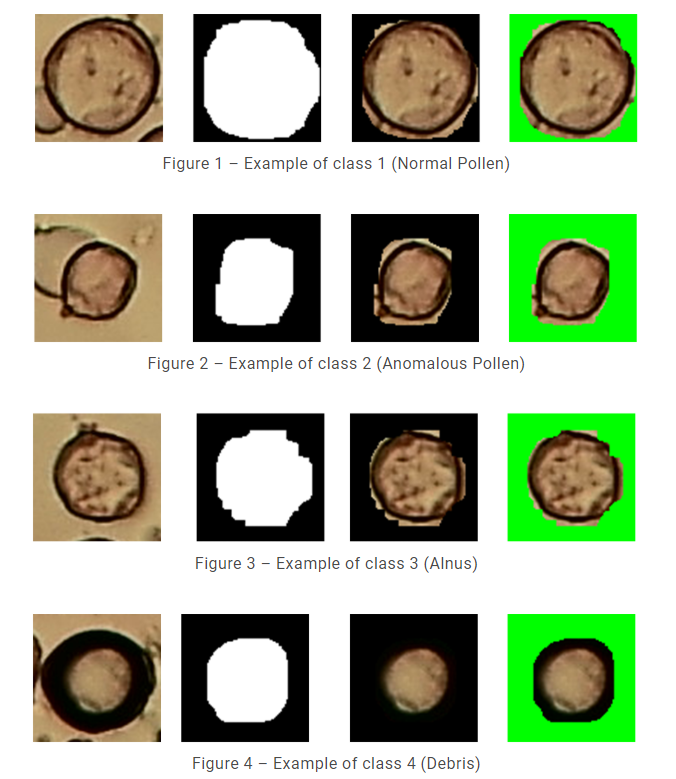
\includegraphics[width = 5in]{../cap5_experimentos/src/polen.png}
    \caption{Imagen extraída de la página oficial del Pollen Challenge \cite{polen}}
\end{figure}
% Métricas
\section{Métricas para clasificación Binaria}
% Accuracy
Analizaremos primero el caso de las métricas en un problema de clasificación binario. Es decir, dada una clase $\mathcal C$, es posible que un dato $y$ pertenezca o no pertenezca a $\mathcal{C}$.

Es importante describir primero las métricas en este tipo de problemas, debido a que cuando nos adentremos a la clasificación multiclase, estas métricas nos serán de utilidad.
\subsection{Matriz de confusión}
Considérese un problema de clasificación binario. En el mejor de los casos, el modelo podría predecir perfectamente qué datos pertenecen a la clase y cuáles no lo hacen. Sin embargo, siendo que es un modelo estadístico, el modelo no siempre acertará, y usando los datos etiquetados se puede detectar en dónde ha habido una \textsl{confusión}. El modelo puede confundirse de dos maneras: La primera es afirmando que $y\in \mathcal C$ cuando no es el caso, y la segunda es clasificar  $y\notin \mathcal C$, cuando en realidad $y$ sí pertenecía a la clase. Por tanto, existen 4 posibilidades:

\begin{enumerate}
    \item \textbf{Verdaderos positivos}: Aquellos datos que sí pertenecen a la clase, y fueron clasificados dentro de la clase. A la cantidad de verdaderos positivos se le denota $T_P$ por sus siglas en inglés.
    \item \textbf{Falsos positivos}: Aquellos datos que sí pertenecen a la clase, y fueron clasificados fuera de la clase. A la cantidad de falsos positivos se le denota $F_P$ por sus siglas en inglés.
    \item \textbf{Verdaderos negativos}: Aquellos datos que no pertenecen a la clase, y fueron clasificados fuera de la clase. A la cantidad de verdaderos negativos se le denota $T_N$ por sus siglas en inglés.
    \item \textbf{Falsos negativos}: Aquellos datos que no pertenecen a la clase, y fueron clasificados dentro de la clase. A la cantidad de falsos negativos se le denota $F_N$ por sus siglas en inglés.
\end{enumerate}
Es posible agrupar toda esta información en una matriz conocida como \textsl{matriz de confusión}. 
\begin{definition}
    \label{pos_neg}
    Considérese el problema de clasificación (\ref{clasification}) con $m = 2$. Sea $f: \mathbb R^n \to C$ el modelo. Definimos los siguientes valores:
    \begin{align*}
        T_P = |\{y_i : c_i &= (1,0)^T \text{ y } f(y_i) = (1,0)^T\}| \\
        F_P = |\{y_i : c_i &= (0,1)^T \text{ y } f(y_i) = (1,0)^T\}| \\
        T_N = |\{y_i : c_i &= (0,1)^T \text{ y } f(y_i) = (0,1)^T\}| \\
        F_N = |\{y_i : c_i &= (1,0)^T \text{ y } f(y_i) = (0,1)^T\}|.
    \end{align*} 
    La matriz de confusión se define como 
    \begin{equation}
        D = \left[\begin{matrix}
            T_P & F_P \\
            F_N & T_N
        \end{matrix}\right].
    \end{equation}
\end{definition}
\begin{figure}[H]
    \centering
    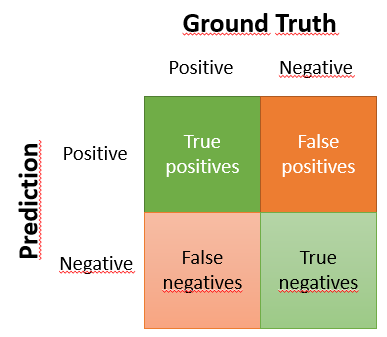
\includegraphics{../cap5_experimentos/src/matriz_confusion_binaria.png}
    \caption{\textcolor{red}{Conseguir imagen propia}}
\end{figure}
%------------- Accuracy
\subsection{Exactitud}
La exactitud se define como la razón de las predicciones acertadas y las predicciones totales. En el aprendizaje automático suele ser la métrica principal, ya que determina el porcentaje de aciertos. Sin embargo, no es el único factor  a tomar en cuenta.
\begin{definition}[exactitud]
    Considérese los valores $T_P, F_P, T_N, F_N$ de la definición (\ref{pos_neg}). La exactitud $A$ se define como 
    \begin{equation}
        A = \frac{T_P + T_N}{T_P + F_P + T_N + F_N}
    \end{equation}
\end{definition}
%------------- Sensibilidad y Especificidad
\subsection{Sensibilidad y Especificidad}
Existen ocasiones en las que no es conveniente utilizar la Exactitud como único criterio del desempeño, especialemente cuando se tiene un conjunto de datos desbalanceado (Sección \ref{unbalanced_sets}). Por ejemplo, al detectar llamadas fraudulentas, no servirá usar la Exactitud, porque casi ninguna llamada es fraudulenta. Lo conveniente sería conocer cuántas veces se acertó al tratar de predecir resultados negativos (Especificidad) o viceversa, cuántas veces se acertó al tratar de predecir resultados positivos (Sensibilidad). 

\begin{definition}
    Considérese los valores $T_P, F_P, T_N, F_N$ de la definición (\ref{pos_neg}). La sensibilidad $R$ y la especificidad $E$ se definen respectivamente como 
    \begin{equation}
        R = \frac{T_P}{T_P + F_P}
    \end{equation}
    \begin{equation}
        E = \frac{T_F}{T_F + F_N}
    \end{equation}
\end{definition}
%------------- Precisión
\subsection{Precisión}
\begin{definition}[Precisión]
    Considérese los valores $T_P, F_P, T_N, F_N$ de la definición (\ref{pos_neg}). La precisión $P$ se define como 
    \begin{equation}
        P = \frac{T_P}{T_P + F_P}
    \end{equation}
\end{definition}
%------------- F1-score
\subsection{\textcolor{red}{F1-score}}
En algunos problemas, es necesario tomar en cuenta la precisión y la sensibilidad por igual. La F1-score, propuesta en 2006 en \cite{f1score}, se define como la media armónica de estas dos métricas. 
\begin{definition}[\textcolor{red}{F1-score}]
    Considérese los valores $T_P, F_P, T_N, F_N$ de la definición (\ref{pos_neg}). La \textcolor{red}{F1-score} $F_1$ se define como 
    \begin{equation}
        F_1  = \frac{2}{\frac{1}{R} + \frac{1}{P}} = \frac{2RP}{R + P} = \frac{T_P}{T_P + \frac{1}{2}(F_P + F_N)}
    \end{equation}
\end{definition}
\begin{figure}[H]
    \centering
    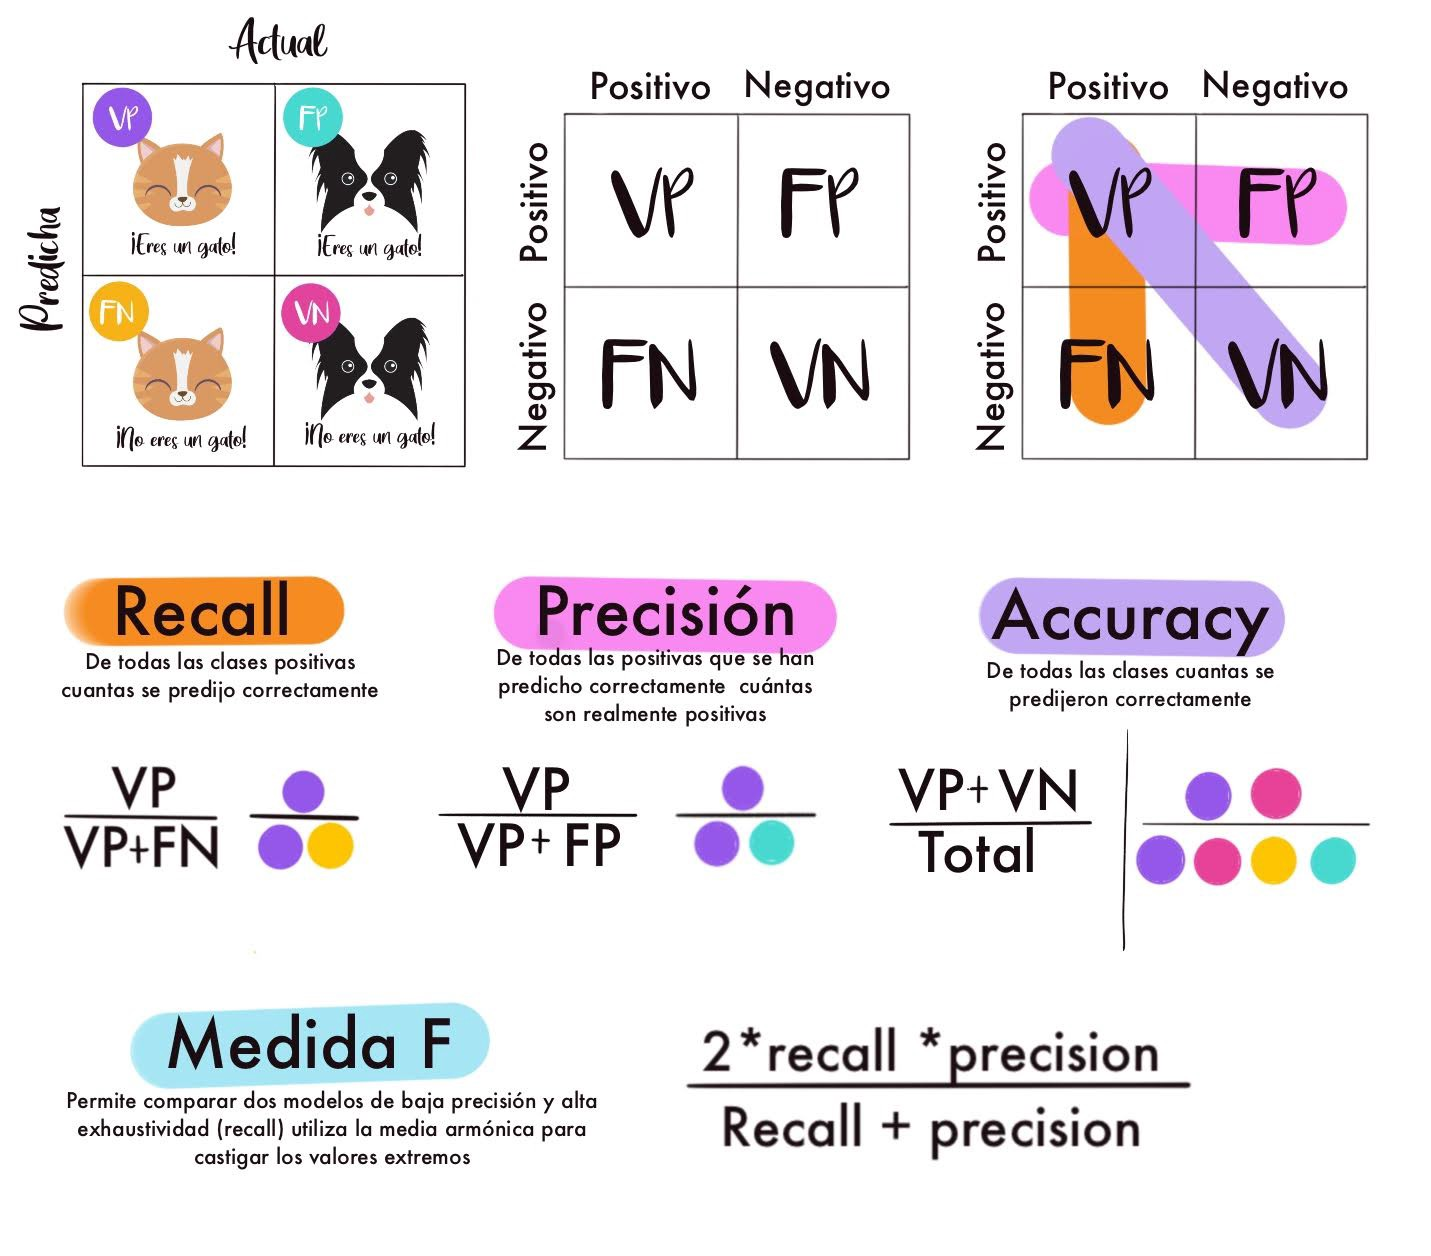
\includegraphics[width=4in]{../cap5_experimentos/src/metricas.jpeg}
\end{figure}
\section{Métricas para clasificación multiclase}
En cuanto a la problema de clasificación con $m$ clases, no podemos hacer uso directo de las todas las fórmulas anteriores. Sin embargo, es posible conseguir una matriz de confusión. En este caso, el eje $x$ determina la verdadera etiqueta, y el eje $y$ determina la etiqueta predicha por el modelo.

De modo que la matriz de confusión para el problema de clasificación multiclase es de la siguiente forma:
\begin{equation}
    D = \left(\begin{matrix}
        d_{1,1} & d_{1,2} & \cdots & d_{1,m} \\
        d_{2,1} & d_{2,2} & \cdots & d_{2,m} \\
        \vdots & \vdots & \ddots & \vdots \\
        d_{m,1} & d_{m,2} & \cdots & d_{m,m} 
    \end{matrix}\right),
\end{equation}
dónde $d_{i,j}$ es la cantidad de elementos pertenecientes a la clase $j$ que fueron clasificados en la clase $i$. Por tanto, un modelo que clasifique todas las instancias correctamente, tendrá una matriz de confusión diagonal.  

\begin{definition}
    Sea $D$ una matriz de confusión, su versión normalizada se determina por la regla 
    \begin{equation}
        \hat d_{i,j} = \frac{d_{i,j}}{|C_i|}
    \end{equation}
\end{definition}

Es sencillo definir la forma generalizada de la Exactitud, basándonos en que es la razón entre la cantidad total de aciertos (La suma de los elementos en la diagonal de la matriz de confusión) y la cantidad total de instancias, es decir la suma de cada entrada de la matriz.
\begin{definition}
    Sea $D$ una matriz de confusión. Se define la exactitud $A$ de la siguiente manera:
    \begin{enumerate}
        \item Exactitud:
        \begin{equation}
            A = \frac{\sum_{i=1}^n d_{i,i}}{\sum_{i,j} d_{i,j}}
        \end{equation} 
    \end{enumerate}
\end{definition}
\begin{figure}[H]
    \centering
    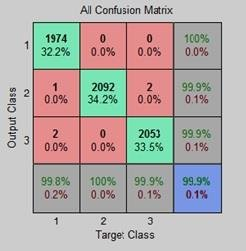
\includegraphics{../cap5_experimentos/src/confision_multiclase.png}
    \caption{\textcolor{red}{Conseguir imagen propia}}
\end{figure}

Por otro lado, para las métricas de Precisión y Sensibilidad se tienen dos posibles definiciones: La \textsl{Macro} y la \textsl{Ponderada}.


 %------------- Macro
 \subsection{Métricas Macro}

 %------------- Ponderada
 \subsection{Métricas Ponderadas}
 
% \input{optimal.tex}
% \appendix
% \input{apendix1.tex}


\bibliographystyle{unsrt}
\bibliography{papers}

\chapter{Notas}
    \begin{enumerate}
        \item La notitas rojas son cosas que aún deben investigarse o cambiarse. Las notas azules representan textos que no están mal, pero que pueden escribirse de una mejor manera.
        \item En preeliminares pretendo definir lo que es una imagen (una función) y un kernel.
    \end{enumerate}

\end{document}